%%%%%%%%%%%%%%%%%%%%%%%%%%%%%%%%%%%%%
%% Master Thesis - Computer Engineering
%% Copyright 2009 Ricardo Alexandre Fiorelli, Erick Poletto
%% This document is distributed by the terms of the license
%% included in the file LICENSE.
%%%%%%%%%%%%%%%%%%%%%%%%%%%%%%%%%%%%%

\documentclass[dvips,ruledheader]{abnt}
% Foi retirado para que o texto fique em inglês
%\usepackage[brazil]{babel}
\usepackage[english]{babel}
\usepackage[latin1]{inputenc}
\usepackage[dvips]{graphicx}
\usepackage{abnt-alf}
\usepackage{latexsym}
\usepackage{psfrag}
\usepackage[center, small, bf]{caption}

% User definined packages
\usepackage{graphicx}
\usepackage{url}
\usepackage{amssymb}
\usepackage{eurofont}
\usepackage{subfig}
\usepackage{tabularx}
\usepackage{rotating}

\setcounter{tocdepth}{2} %To set the depth for numbering for the Table of Contents

% Use defined commands
\newcommand{\tn}{\tabularnewline}
\newcommand{\tnhl}{\tabularnewline\hline}

\begin{document}

\DeclareGraphicsRule{.eps.gz}{eps}{.eps.bb}{`gunzip -c #1}

%\include{capa}
%%%%%%%%%%%%%%%%%%%%%%%%%%%%%%%%%%%%%
%% Master Thesis - Computer Engineering
%% Copyright 2009 Ricardo Alexandre Fiorelli, Erick Poletto
%% This document is distributed by the terms of the license
%% included in the file LICENCE.
%%%%%%%%%%%%%%%%%%%%%%%%%%%%%%%%%%%%%

%%%%%%%%%%%%%%%%%%%%%%%%%%%%%%%%%%%%%
%% Coverpage
%%%%%%%%%%%%%%%%%%%%%%%%%%%%%%%%%%%%%

% Usando o comando \capa

\titulo{Title of the Thesis} % TODO

\autor{Erick Poletto \\ Ricardo Alexandre Fiorelli}

\orientador[Orientator:]{Prof. Chiara Francalanci}
% ou \orientador[Orientadora:\\]{Minha orientadora}

%\coorientador{Meu co-orientador}
% ou \coorientador[Co-orientadora:\\]{Minha co-orientadora}

\comentario{comments}% TODO


\instituicao{Master Thesis in Computer Engineering \par 
	Dipartimento di Elettronica ed Informazione (DEI)\par 
	Politecnico di Milano}

\local{Milan -- IT}

\data{July/2009}

\capa


% ou...
% fazendo a mao
%
% \begin{titlepage}
%
%   ... codigo da folha de rosto
%  
% \end{titlepage}


%%%%%%%%%%%%%%%%%%%%%%%%%%%%%%%%%%%%%%
%% Master Thesis - Computer Engineering
%% Copyright 2009 Ricardo Alexandre Fiorelli, Erick Poletto
%% This document is distributed by the terms of the license
%% included in the file LICENCE.
%%%%%%%%%%%%%%%%%%%%%%%%%%%%%%%%%%%%%

%%%%%%%%%%%%%%%%%%%%%%%%%%%%%%%%%%%%%
%% Folha de rosto
%%%%%%%%%%%%%%%%%%%%%%%%%%%%%%%%%%%%%

% Usando o comando \folhaderosto

\titulo{Title of the Thesis}

\autor{Erick Poletto // Ricardo Alexandre Fiorelli}

\begin{center}
Copyright 2009 Ricardo Alexandre Fiorelli, Erick Poletto.\\ This document is distributed by the terms of the license included in the file LICENCE.
\end{center}

\orientador{Prof. Chiara Francalanci}
% ou \orientador[Orientadora:\\]{Minha orientadora}

%\coorientador{Meu co-orientador}
% ou \coorientador[Co-orientadora:\\]{Minha co-orientadora}

\comentario{Disserta��o apresentada � Coordena��o do Mestrado em Engenharia e Ci�ncia de Materiais da Universidade Federal do Cear� para a obten��o do t�tulo de Mestre em Engenharia e Ci�ncia de Materiais.}


\instituicao{Master Thesis in Computer Engineering \par 
	Dipartimento di Elettronica ed Informazione (DEI)\par 
	Politecnico di Milano}

\local{Milan -- IT}

\data{July/2009}


\folhaderosto


% ou...
% fazendo a mao
%
% \begin{titlepage}
%
%   ... codigo da folha de rosto
%  
% \end{titlepage}

%%%%%%%%%%%%%%%%%%%%%%%%%%%%%%%%%%%%%
%% Master Thesis - Computer Engineering
%% Copyright 2009 Ricardo Alexandre Fiorelli, Erick Poletto
%% This document is distributed by the terms of the license
%% included in the file LICENCE.
%%%%%%%%%%%%%%%%%%%%%%%%%%%%%%%%%%%%%

%%%%%%%%%%%%%%%%%%%%%%%%%%%%%%%%%%%%%
%% Folha de rosto
%%%%%%%%%%%%%%%%%%%%%%%%%%%%%%%%%%%%%

% Usando o comando \folhaderosto

\titulo{Title of the Thesis}

\autor{Erick Poletto // Ricardo Alexandre Fiorelli}

\begin{center}
Copyright 2009 Ricardo Alexandre Fiorelli, Erick Poletto.\\ This document is distributed by the terms of the license included in the file LICENCE.
\end{center}

\orientador{Prof. Chiara Francalanci}
% ou \orientador[Orientadora:\\]{Minha orientadora}

%\coorientador{Meu co-orientador}
% ou \coorientador[Co-orientadora:\\]{Minha co-orientadora}

\comentario{Disserta��o apresentada � Coordena��o do Mestrado em Engenharia e Ci�ncia de Materiais da Universidade Federal do Cear� para a obten��o do t�tulo de Mestre em Engenharia e Ci�ncia de Materiais.}


\instituicao{Master Thesis in Computer Engineering \par 
	Dipartimento di Elettronica ed Informazione (DEI)\par 
	Politecnico di Milano}

\local{Milan -- IT}

\data{July/2009}


\folhaderosto


% ou...
% fazendo a mao
%
% \begin{titlepage}
%
%   ... codigo da folha de rosto
%  
% \end{titlepage}


%%%%%%%%%%%%%%%%%%%%%%%%%%%%%%%%%%%%%%
%% Master Thesis - Computer Engineering
%% Copyright 2009 Ricardo Alexandre Fiorelli, Erick Poletto
%% This document is distributed by the terms of the license
%% included in the file LICENCE.
%%%%%%%%%%%%%%%%%%%%%%%%%%%%%%%%%%%%%

%%%%%%%%%%%%%%%%%%%%%%%%%%%%%%%%%%%%%
%% 
%%%%%%%%%%%%%%%%%%%%%%%%%%%%%%%%%%%%%

\begin{folhadeaprovacao}
Disserta��o de Mestrado sob o t�tulo \textit{``Avalia��o da qualidade da gasolina atrav�s de medidas el�tricas''}, defendida por Dehon Charles Regis Nogueira e aprovada em 17 de janeiro de 2003, em Fortaleza, Cear�, pela banca examinadora constitu�da pelos doutores:

\setlength{\ABNTsignthickness}{0.4pt}
\setlength{\ABNTsignwidth}{10cm}
\setlength{\ABNTsignskip}{3.5cm}

\assinatura{Prof. Dr. Ant�nio S�rgio Bezerra Sombra \\ Departamento de F�sica - UFC \\ Orientador}

\assinatura{Prof. Dr. Hamilton Ferreira Gomes de Abreu \\ Departamento de Engenharia Mec�nica - UFC}

\assinatura{Prof. Dr. Edval Jos� Pinheiro Santos \\ Departamento de Eletr�nica e Sistemas - UFPE}

\end{folhadeaprovacao}


%%%%%%%%%%%%%%%%%%%%%%%%%%%%%%%%%%%%%%
%% Master Thesis - Computer Engineering
%% Copyright 2009 Ricardo Alexandre Fiorelli, Erick Poletto
%% This document is distributed by the terms of the license
%% included in the file LICENCE.
%%%%%%%%%%%%%%%%%%%%%%%%%%%%%%%%%%%%%

%%%%%%%%%%%%%%%%%%%%%%%%%%%%%%%%%%%%%
%% Dedicatoria
%%%%%%%%%%%%%%%%%%%%%%%%%%%%%%%%%%%%%

\ 

\vfill

\begin{flushright}
\hfill \textit{que bonitinho\ldots}
\end{flushright}

\vspace*{1cm}

\clearpage

%%%%%%%%%%%%%%%%%%%%%%%%%%%%%%%%%%%%%
%% Master Thesis - Computer Engineering
%% Copyright 2009 Ricardo Alexandre Fiorelli, Erick Poletto
%% This document is distributed by the terms of the license
%% included in the file LICENCE.
%%%%%%%%%%%%%%%%%%%%%%%%%%%%%%%%%%%%%

%%%%%%%%%%%%%%%%%%%%%%%%%%%%%%%%%%%%%
%% Dedicatoria
%%%%%%%%%%%%%%%%%%%%%%%%%%%%%%%%%%%%%

\ 

\vfill

\begin{flushright}
\hfill \textit{que bonitinho\ldots}
\end{flushright}

\vspace*{1cm}

\clearpage


%%%%%%%%%%%%%%%%%%%%%%%%%%%%%%%%%%%%%%
%% Master Thesis - Computer Engineering
%% Copyright 2009 Ricardo Alexandre Fiorelli, Erick Poletto
%% This document is distributed by the terms of the license
%% included in the file LICENCE.
%%%%%%%%%%%%%%%%%%%%%%%%%%%%%%%%%%%%%

%%%%%%%%%%%%%%%%%%%%%%%%%%%%%%%%%%%%%
%% Acknowledgements
%%%%%%%%%%%%%%%%%%%%%%%%%%%%%%%%%%%%%

\chapter*{Acknowledgements}


% Agradecimentos - � so para as pessoas que contribuiram relevantemente
% para a elabora��o do trabalho

Dedico meus sinceros agradecimentos para:

-- To professor Chiara Francalanci, blah blah blah
% TODO

%%%%%%%%%%%%%%%%%%%%%%%%%%%%%%%%%%%%%
%% Master Thesis - Computer Engineering
%% Copyright 2009 Ricardo Alexandre Fiorelli, Erick Poletto
%% This document is distributed by the terms of the license
%% included in the file LICENCE.
%%%%%%%%%%%%%%%%%%%%%%%%%%%%%%%%%%%%%

%%%%%%%%%%%%%%%%%%%%%%%%%%%%%%%%%%%%%
%% Acknowledgements
%%%%%%%%%%%%%%%%%%%%%%%%%%%%%%%%%%%%%

\chapter*{Acknowledgements}


% Agradecimentos - � so para as pessoas que contribuiram relevantemente
% para a elabora��o do trabalho

Dedico meus sinceros agradecimentos para:

-- To professor Chiara Francalanci, blah blah blah
% TODO


%%%%%%%%%%%%%%%%%%%%%%%%%%%%%%%%%%%%%%
%% Master Thesis - Computer Engineering
%% Copyright 2009 Ricardo Alexandre Fiorelli, Erick Poletto
%% This document is distributed by the terms of the license
%% included in the file LICENCE.
%%%%%%%%%%%%%%%%%%%%%%%%%%%%%%%%%%%%%

%%%%%%%%%%%%%%%%%%%%%%%%%%%%%%%%%%%%%
%% Epigrafe
%%%%%%%%%%%%%%%%%%%%%%%%%%%%%%%%%%%%%


%  Ep�grafe - � uma cita��o pertinente ao seu trabalho
%  ou que represente o seu modo de pensar. 
%  Resumindo, coloque uma frase que o(a) agrade.


\pretextualchapter{}

\vspace{17.5cm}
\begin{flushright}

\textit{``A atividade da engenharia, enquanto permanecer atividade, \\
	 pode levar a criatividade do homem a seu grau m�ximo; \\
	 mas, assim que o construtor p�ra de construir e se entrincheira \\
	 nas coisas que fez, as energias criativas se congelam, \\
	 e o pal�cio se transforma em tumba.'' \\ 
	\bfseries Marshall Berman}

\end{flushright}



%%%%%%%%%%%%%%%%%%%%%%%%%%%%%%%%%%%%%
%% Master Thesis - Computer Engineering
%% Copyright 2009 Ricardo Alexandre Fiorelli, Erick Poletto
%% This document is distributed by the terms of the license
%% included in the file LICENCE.
%%%%%%%%%%%%%%%%%%%%%%%%%%%%%%%%%%%%%

%%%%%%%%%%%%%%%%%%%%%%%%%%%%%%%%%%%%%
%% Epigrafe
%%%%%%%%%%%%%%%%%%%%%%%%%%%%%%%%%%%%%


%  Ep�grafe - � uma cita��o pertinente ao seu trabalho
%  ou que represente o seu modo de pensar. 
%  Resumindo, coloque uma frase que o(a) agrade.


\pretextualchapter{}

\vspace{17.5cm}
\begin{flushright}

\textit{``A atividade da engenharia, enquanto permanecer atividade, \\
	 pode levar a criatividade do homem a seu grau m�ximo; \\
	 mas, assim que o construtor p�ra de construir e se entrincheira \\
	 nas coisas que fez, as energias criativas se congelam, \\
	 e o pal�cio se transforma em tumba.'' \\ 
	\bfseries Marshall Berman}

\end{flushright}




%%%%%%%%%%%%%%%%%%%%%%%%%%%%%%%%%%%%%
%% Master Thesis - Computer Engineering
%% Copyright 2009 Ricardo Alexandre Fiorelli, Erick Poletto
%% This document is distributed by the terms of the license
%% included in the file LICENCE.
%%%%%%%%%%%%%%%%%%%%%%%%%%%%%%%%%%%%%

%%%%%%%%%%%%%%%%%%%%%%%%%%%%%%%%%%%%%
%% tirar esse arquivo
%% Questions and Doubts
%%%%%%%%%%%%%%%%%%%%%%%%%%%%%%%%%%%%%

\chapter*{Questions and Doubts}
    In order not to have any text not related to the thesis in the middle of the text and maybe, in the final version nobody sees it, I created this file, like that, we can put some information here and delete it in the last version. Of course, these are not the only issues related to the thesis, but it is better to have a centralized way to do that.

    The questions are:
\begin{description}
	\item [Section~\ref{sec3:components_database} or Appendix~\ref{app:sandra_benchmark_table_schema}] Do we need to insert all tables here, in appendix, or where do we need to insert the tables? Or just the database schema? These tables were taken from the SANDRA Access file.
\end{description}
 %XXX tirar essa parte na versao final da tese

%%%%%%%%%%%%%%%%%%%%%%%%%%%%%%%%%%%%%
%% Master Thesis - Computer Engineering
%% Copyright 2009 Ricardo Alexandre Fiorelli, Erick Poletto
%% This document is distributed by the terms of the license
%% included in the file LICENCE.
%%%%%%%%%%%%%%%%%%%%%%%%%%%%%%%%%%%%%

%%%%%%%%%%%%%%%%%%%%%%%%%%%%%%%%%%%%%
%% Abreviations
%%%%%%%%%%%%%%%%%%%%%%%%%%%%%%%%%%%%%

\chapter*{Glossary of Abrevitations}


% Abreviações dos termos usados no trabalho

\begin{center}
	\begin{tabular}{|l|l|} \hline
	    x       &   x                                           \tnhl
	    CPU     &   Central Processing Unit                     \tnhl
	    DDR     &   Double-Data Rate                            \tnhl
        HVAC    &                                               \tnhl
	    HDD     &   Hard-disk Drive                             \tnhl
	    ICT     &   Information and Communcation Technology     \tnhl
	    LTO     &   Linear Tape-Open                            \tnhl
		MFD     &   Multi Function Devices                      \tnhl
    	MPN     &   Manufacturer Part Number                    \tnhl
    	OS      &   Operational System                          \tnhl
    	PC      &   Personal Computer                           \tnhl
    	PDU     &                                               \tnhl
    	PSU     &   Power Supply Unit                           \tnhl
    	RAID    &                                               \tnhl
		ROI     &   Return on Investment                        \tnhl
		ROM     &   Read-Only Memory                            \tnhl
		SaaS    &   Software as a Service                       \tnhl
		SDRAM   &   Synchronous Dynamic Random Access Memory    \tnhl
		SAN     &   Storage-Area Networks                       \tnhl
		TOC     &   Total Cost of Ownership                     \tnhl
		VM      &   Virtual Machine                             \tnhl
		x       &   x                                           \tnhl
	\end{tabular}
	\label{tab:glossary_of_abbreviations}
\end{center}
% TODO


%%%%%%%%%%%%%%%%%%%%%%%%%%%%%%%%%%%%%
%% Master Thesis - Computer Engineering
%% Copyright 2009 Ricardo Alexandre Fiorelli, Erick Poletto
%% This document is distributed by the terms of the license
%% included in the file LICENCE.
%%%%%%%%%%%%%%%%%%%%%%%%%%%%%%%%%%%%%

%%%%%%%%%%%%%%%%%%%%%%%%%%%%%%%%%%%%%
%% Abstract
%%%%%%%%%%%%%%%%%%%%%%%%%%%%%%%%%%%%%


\begin{abstract} 
\label{abstract}
% Apresenta��o concisa dos pontos relevantes, dando uma visao rapida e
% clara do conte�do do trabalho.


%%%%%%%%%%%%
%% Importante: Os comentarios abaixo, somente separam cada parte do abstract, porem, nao devem ser 
%% separados, pois trata-se de somente um paragrafo
%%%%%%%%%%%%

%%%Parts of the abstract
%%%Rationale
Since the last few years cost of energy has become an important part of Data Centers total cost of ownership. This has lead organizations worldwide to recognize the importance of a green strategy as a means to save energy and reduce the cost of maintenance.
%%%Objectives
This study was conducted in order to catalog computer components related data by means of benchmarking and web research. With the objective of designing a component's database and then the power-related data obtained from the used benchmarking tools was validated with the use of direct measurements.
%%%Methods
The data acquired for composing this database of components was obtained from different sources, which were both a benchmarking tool and the web. The benchmarking tool provided information about component performance and power consumption. After that, a web crawler was used to assign each component an unique key and to provide additional information about them.
%%%Results
This work provided a database of components which can be used to support a green ICT methodology by allowing the identification of the most adequate and power-efficient components, and also the analysis of this benchmarking tool.
%%%Conclusions
It provides for the individuation of energy consumption critical spots in a data center and allows comparisons between several components, which may both be used in data center design.

\end{abstract}




\tableofcontents

\listoffigures
\listoftables

%\include{motivacao}
%%%%%%%%%%%%%%%%%%%%%%%%%%%%%%%%%%%%%
%% Master Thesis - Computer Engineering
%% Copyright 2009 Ricardo Alexandre Fiorelli, Erick Poletto
%% This document is distributed by the terms of the license
%% included in the file LICENCE.
%%%%%%%%%%%%%%%%%%%%%%%%%%%%%%%%%%%%%

%%%%%%%%%%%%%%%%%%%%%%%%%%%%%%%%%%%%%
%% First Chapter
%% Motivation
%%%%%%%%%%%%%%%%%%%%%%%%%%%%%%%%%%%%%

% \chapter*{Motivation} \label{motivation}

% Mostrar o que levou a realiza��o do trabalho, e as motiva��es para que o problema seja entendido.
% Situa��o do leitor no contexto
%O greenict tem sido muito importatne para o mundo, as empresas, depois da crise economica, comecaram a ver que é importante, pois, reduz muitos custos, além de contribuirem apra o meio ambiente\ldots bla bla bla

    %TODO
    





%%%%%%%%%%%%%%%%%%%%%%%%%%%%%%%%%%%%%
%% Master Thesis - Computer Engineering
%% Copyright 2009 Ricardo Alexandre Fiorelli, Erick Poletto
%% This document is distributed by the terms of the license
%% included in the file LICENCE.
%%%%%%%%%%%%%%%%%%%%%%%%%%%%%%%%%%%%%

%%%%%%%%%%%%%%%%%%%%%%%%%%%%%%%%%%%%%
%% First Chapter
%% Introduction
%%%%%%%%%%%%%%%%%%%%%%%%%%%%%%%%%%%%%


\chapter{Introduction} \label{chap1:introduction}


%     This is a general introduction to what the thesis is all about – it is ust a description of the contents
% of each section. Briefly summarize the question (you will be stating the question in detail later),
% some of the reasons why it is a worthwhile question, and perhaps give an overview of your main
% results. This is a birds-eye view of the answers to the main questions answered in the thesis (see
% above).

\section{Motivation} \label{sec1:motivation}
% Mostrar o que levou a realiza��o do trabalho, e as motiva��es para que o problema seja entendido.
% Situa��o do leitor no contexto
%O greenict tem sido muito importatne para o mundo, as empresas, depois da crise economica, comecaram a ver que é importante, pois, reduz muitos custos, além de contribuirem apra o meio ambiente\ldots bla bla bla

% o consumo nao eh de 25% do que o planeta ainda tem. mas sim de 125% do que ele pode renovar a cada ano... esse eh o valor fixo, nao a taxa de crescimento
    The planet is threatened by global warming. The progressive pressure we impose to the environment has already exceeded the limits imposed by the available natural resources. In actual figures, it can be stated that 125\% of the renewal capacity of natural resources is currently consumed. If the growth continues at this rate, in 2050 we will be consuming more than twice the production capacity of the planet Earth~\cite{Townsend:2002:2050}. 
    
    The seek for environmental friendly solutions is spreading throughout all the economic sectors and consumers have become more aware of environmental issues and thus opt for products and services of companies which have proven to be more ecologically friendly. Moreover, it is possible to say that we will soon enter in a green trend - if we are not already in it - where environmental policies will be executed without economical or political pressure, but rather as a necessary measure for the sustainability of the business. In a following phase companies will perceive green solutions as a competitive differential instead of a necessary preoccupation thereby giving the green issue a push towards being a definitive part of the business.
        
    In the last years, the concept of Green ICT has been increasingly popular by the mantra of \emph{Going Green}. A study from Info-Tech Research Group~\cite{info-tech07}, made in U.S.A., believes that the increasing interest in adopting a green solution is beginning to generate meaningful actions. However, there exists a big gap between what companies think it is a green ICT solution and what they are really doing about it. This same study states that ``Info-Tech expects continued interest in green IT strategies and significant traction among those initiatives that both reduce waste and reduce cost. As enterprises begin to translate concern for green into practice, we expect higher spending in many leading areas such as data center design, virtualization and consolidation, print optimization, and system management tools''.
    
    The current situation is that there exists a high interest in the issue, yet scarce adoption. Nonetheless, companies have reached the consensus that it is necessary to start changing their minds towards green thoughts. So, leading industries and governments have started a proactive \emph{Going Green} promotion to expand the existent market. Measures taken in favor of this green market include the allocation of a significant amount of money in researches in the area. Besides that, it is important to notice that as soon as information related of careful management of energy consumption starts to spread, it will start to attract the companies attention. The first step will be to start to study the impact of environmental harm and power consumption in the TCO accountancies.
    
    The most important benefit of a Green ICT strategy is the reduction of costs related to the energy consumption. Some studies says that the costs with power and cooling in data centers can reach up to 20\% of the IT cost. In the economic sector, the potential savings for companies could be huge and simple actions can have big impacts in the organization. As David Frampton, VP general manager of Cisco's LAN switching business unit, explained to Reuters~\cite{Chestney2009}, "a bank branch could save nearly \euro40,000 (US\$53,020) just by turning off phones and wireless access points outside business hours". Following the same pattern, last year, Symantec launched a study named ``State of the Data Center Report 2008'', in which the social responsibility was the least important reason for applying a Green initiative. It states instead that \emph{reduction of costs} and \emph{reduction of power consumption} are the most important reasons to invest in such idea. 
    
    Another benefit is that Green ICT can be used as a \emph{marketing strategy} and with the growing popularity of the issue, vendors have started to put green labels on their products and consumers also started to seek for green products instead of the traditional ones. And if the scenario continues like that, the companies which do not adopt the \emph{Going Green} concept will lose an important competitive edge.
    
    The most difficult phase when applying a new solution is going against the inertia of the company. In this case, the state of being at rest is not applying a green solution and what is required is the force and influence for pushing forward the green idea. After the first step has been taken the others should come with time. A critical issue for taking this first step towards the green initiative is the allocation of budget. Before the economical crisis IT resources could be larger, but now it has become more difficult to manage the budget towards new initiatives. Therefore, the Green ICT budget should reflect what the company is expecting from the solution. Even with the economical crisis, there has been an increase in the expenses with technology production related to power efficient products, which usually is allied with productivity increase and reduction of waste generation. 
    
        This work relates to one specific aspect of the \emph{Going Green} concept, which is the \emph{Green Data Center}. The related measures focuses in re-engineering the Data Center with the use of a wide number of techniques that will be described in the following chapter.

%    Portanto, as empresas que investem em datacenter especializados podem esperar um contínuo processo de modernização, já que este mercado investe constantemente em soluções de consolidação e virtualização de servidores, storage e equipamentos de rede, além de blade, a grande tendência do momento.

% \section{Terminology Clarification} \label{sec1:terminology_clarification}
%TODO  OPTIONAL
%     A brief section giving background information may be necessary, especially if your work spans
% two or more traditional fields. That means that your readers may not have any experience with
% some of the material needed to follow your thesis, so you need to give it to them. A different title
% than that given above is usually better; e.g., ”Frammis Algebra.”


\section{Definition of the problem} \label{sec1:problem}

    The present study was conducted in order to empirically and quantitatively catalog computer components related data by means of benchmarking, web research and to validate these with the use of direct measurements. This information can then be used to better compose the data center with respect to energy efficiency. The goal is to support companies in order to apply a green solution by assisting the choice of the right combination of components and, besides that, point the ones which consumes less energy and have higher efficiency (best performance/power ratio).
    
    Moreover, this study may provide a means to identify critical bottlenecks in power consumption and to address the problem by making a more efficient use of the identified components. To that end, the aim of this research is to design a computer component database with information about their characteristics and benchmark tests. The information that regards power consumption will then be validated with the use of direct measurements in order to determine the accuracy of the component power estimated by the benchmarking tools.
    
    \subsection{Thesis Statement}\label{sec1:thesis_statement}
        The study aims to address the following questions:
        \begin{enumerate}
	        \item Which computer components are more efficient, i.e. consume the less energy while providing a good performance?
	        \item How to choose among a set of machine configurations the best one, concerning power efficiency?
	        \item How to catalog, analyze and understand the reasons behind power efficiency in a component?
        \end{enumerate}
        
    These will be addressed with the use of an adequate component database, which will be the scope of this work.

\section{Solution Strategy} \label{sec1:solution_strategy}

    The first step to be taken in the direction of the solution to the problem is data collection. In this phase, it was acquired from many sources, that will be described in Chapter~\ref{chap3:methodology}, data related to the energy consumed by the components. After this, the information collected was separated by categories and linked together with a MPN code, which is unique for each component. All the information acquired from the measures was inserted into a consolidated database of components. The next step is the analysis of the collected data. This \emph{database of components} has as objective finding a \emph{qualitative solution} to the issue of choosing the best machine configuration concerning their energy efficiency.

\section{Structure} \label{sec1:structure}

% colocar a estrutura dos capitulos e do documento...
    This document is structured as follows:
    \begin{itemize}
        \item Chapter~\ref{chap1:introduction} is the introduction;
        \item Chapter~\ref{chap2:state_of_the_art} is the state of the art, giving relevant information about available technologies and techniques applied in Green ICT;
        \item Chapter~\ref{chap3:methodology} is the Methodology, where the problem is engineered, the used method used is exposed and a means to evaluate it is provided;
        \item Chapter~\ref{chap4:analysis_results} exposes the results achieved. It describes how the database was created and explains the results of the analysis carried out to evaluate it;
        \item Chapter~\ref{conclusion} is the conclusion. It presents the conclusion of the work and suggests how it could be further developed.
    \end{itemize}
    
    

%%%%%%%%%%%%%%%%%%%%%%%%%%%%%%%%%%%%%
%% Master Thesis - Computer Engineering
%% Copyright 2009 Ricardo Alexandre Fiorelli, Erick Poletto
%% This document is distributed by the terms of the license
%% included in the file LICENCE.
%%%%%%%%%%%%%%%%%%%%%%%%%%%%%%%%%%%%%

%%%%%%%%%%%%%%%%%%%%%%%%%%%%%%%%%%%%%
%% Second Chapter
%% State of the Art
%%%%%%%%%%%%%%%%%%%%%%%%%%%%%%%%%%%%%

\chapter{State of the Art} \label{chap2:state_of_the_art}
    \section{Green ICT or Green Computing} \label{sec2:green_ict}
		Green ICT, which is a new term originated from ``Green Computing'', is the exploitation of a combination of techniques and approaches in ICT towards the end of achieving a more energy efficient use of computer related resources. In other words, it is the research and development of techniques and software that monitor the energy spent by servers, computers, printers and all information and communication equipment to the end of making a responsible use of these resources in terms of energy consumption. In order to achieve this objective, it is imperative to analyse the information about the ICT components among workstations, servers, networks, cooling and many others. The analysis of the information provided by these measures is made through a set of tools, which will be explained in the chapter~\ref{chap3:methodology}.        

		The steps that have to be taken in order to apply a green strategy are first to analyse where in the data center the more energy is being wasted (``Assessment''), and then to act with correction and prevention interventions (``Action Plan''). For instance: when buying a new piece of equipment, it should be determined how much energy each of the available options spend and opt for those which consume less energy. Moreover, energy-efficient architectures such as thin clients, virtualization and power management policies should be considered in higher decisional levels. The direct benefits from green ICT strategies range from the direct reduction of electricity bills and costs related to cooling to the reduction of the space required by a datacenter.

		The ICT energy consumption has become a critical issue for IT organizations nowadays, where it can provide substantial cost reductions in datacenters and compliance with environmental policies. In the United States alone, data centers consumed \$4.5 billion worth of electricity in 2006. Industry analyst Gartner~\cite{GartnetKumar07} estimates that over the next 5 years, most enterprises will spend as much energy as they spend on hardware infrastructure, power and air conditioning. Furthermore, It is also important to consider that there are some indirect objectives concerning green computing, such as reduction of carbon footprint and disposal of hazard elements to the environment.
		In the next section there is the explanation of all the approaches and categories for applying a green solution.
        
        \subsection{Strategies for Applying a Green Solution} \label{sec2:strategies_applying_green_solution}
            According to NTT Communications\footnote{\url{http://www.ntt.com/business_e/feature/green_ict.html}}, there are two main approaches for applying a green solution.
            \begin{description}
            	\item[Green of ICT] concentrates on the operation of the ICT equipment and information system. The objective of the method is to reduce the environmental through power savings and recycling.
                	\begin{description}
                		\item[Data Center] Centralizing the information in a Data Center, with consolidated data, thereby reducing power consumption whereas improve the efficiency regarding cost, operation adn maintenance.
                		\item[Hosting] It is a enterprise related solution including virtualization, by optimally allocating the resources.
                	\end{description}
            	\item[Green by ICT] concentrates on the energy efficiency reached by the use of ICT operations. The objective is to reduce logistics and transport movements through ICT. Also, reducing material consumption.
            	    \begin{description}
            	    	\item[Communitation] reduces the energy consumed with transportation, by utilizing VOIP solutions with video-conference
            	    	\item[Remote Data Access] reduction of travel and material consumption by having, for example, mobile terminals or VPNs, where the employees can have acces to work information wherever. In addition, the service should provide secure and reliable remote access enabling the use of multiple devices.
            	    \end{description}
            \end{description}

    \section{Computer Energy Management Categories} \label{sec2:energy_categories}

    In terms of hardware and equipment, the main measures to be taken towards a Green ICT environment can be grouped in the following categories:
    \begin{itemize}
        \item Workstation Configuration;
        \item Policies / Tools / Labels;
        \item Thin client architectures;
        \item Servers and Virtualization;
        \item Data Storage;
        \item Power Architectures;
        \item Data Center Infrastructure.
    \end{itemize}
    For each of those categories there are several types of information that are relevant to the evaluation of the current situation of power consumption. For each category there will be a corresponding description along with a number of possible interventions, either purely conceptual or available in the market.In some cases a numerical analysis will also be provided. This information will allow the creation of a methodology to identify critical consumption issues where an investment in green ICT would bring the greater savings.
    
    \subsection{Machine Configuration}\label{sec2:machine_configuration}
        This category represents the components used in a certain machine configuration. The component's performance and power consumption can be obtained from several sources, such as the manufacturer specifications, benchmarks and also direct measurements in the case of power consumption.
        The following are the dimensions that influence the final power consumption of a machine.
            \paragraph*{Single-core / Multi-core Processors} Processors in general affect the overall power consumption of the computer by means of the workload that is required by it. For example, if the computer is in idle (without any processes running) the energy consumed is less than if the computer stays in full workload, but the idle state does not mean anything to the efficiency, because it is needed a high workload (about 70\%) to have the best workload/power consumption ratio.
            %Tirei o cache pelo simples fato de que nao afeta na overall consumption
            %\paragraph*{Cache Memory} %TODO Type and dimension of 
            \paragraph*{RAM Memory} There are several types and dimensions of memories that should be analyzed, for instance the difference in operation in 2.5V in DDR SDRAM, when compared 3.3V in SDRAM significantly reduce the power consumption. When compating DDR and DDR2, The Table~\ref{tab:power_consumption_ram}\nocite{Cooke:2009:Online} compares the difference in power consumption of DDR and DDR2 under various circumstances and it shows that the power consumed by RAM, even on maximum workload (+4.5W), does not have much effect on the overall computer consumption (~220W).
				\begin{table}[h!tb]
				\centering \resizebox{\textwidth}{!}{ % Fazendo a tabela caber no espaco da pagina
				\begin{tabular}{|c|c|c|c|c|c|c|}
				\hline
				\textbf{RAM Type } & \textbf{Size } & \textbf{Load } & \textbf{+12V1 } & \textbf{+5V } & \textbf{+3.3V } & \textbf{Rise from Baseline } \tnhl
				\multicolumn{ 1}{|c|}{\textbf{PC3200 DDR }} & \multicolumn{ 1}{c|}{512 MB } & Idle  & 0.5A  & 0.6A  & 3.0A  & n/a  \tn \cline{ 3- 7}
				\multicolumn{ 1}{|c|}{} & \multicolumn{ 1}{c|}{} & Memtest86  & No Change  & No Change  & +0.7A  & +2.3W  \tn \cline{ 2- 7}
				\multicolumn{ 1}{|c|}{} & \multicolumn{ 1}{c|}{1 GB} & Idle  & No Change  & No Change  & +0.6A  & +2.0W  \tn \cline{ 3- 7}
				\multicolumn{ 1}{|c|}{} & \multicolumn{ 1}{c|}{} & Memtest86  & No Change  & No Change  & +1.0A  & +3.3W  \tnhl
				\multicolumn{ 1}{|c|}{\textbf{533 MHz DDR2 }} & \multicolumn{ 1}{c|}{512 MB } & Idle  & 0.5A  & 3.6A  & 0.5A  & n/a  \tn \cline{ 3- 7}
				\multicolumn{ 1}{|c|}{} & \multicolumn{ 1}{c|}{} & Memtest86  & No Change  & +0.4A  & No Change  & +2.0W  \tn \cline{ 2- 7}
				\multicolumn{ 1}{|c|}{} & \multicolumn{ 1}{c|}{1 GB} & Idle  & No Change  & No Change  & No Change  & No Change  \tn \cline{ 3- 7}
				\multicolumn{ 1}{|c|}{} & \multicolumn{ 1}{c|}{} & Memtest86  & No Change  & +0.9A  & No Change  & +4.5W \tnhl
				\end{tabular}}
				\caption{Power Consumption: RAM}
				\label{tab:power_consumption_ram}
				\end{table}
            \paragraph*{Hard Drives and Mass Memory} Power consumption in this case is affected mainly by design of the hard drive's spindle motor and the number and size of the spindle platters and, also,other components such as the actuator and controller board. Also, solid-state and flash drives reduce significantly the power consumed by the component, Figure~\ref{fig:power_consumption_harddrive} shows this difference.%XXX melhorar essa parte
                \begin{figure}[h!tb]
                    \centering
                    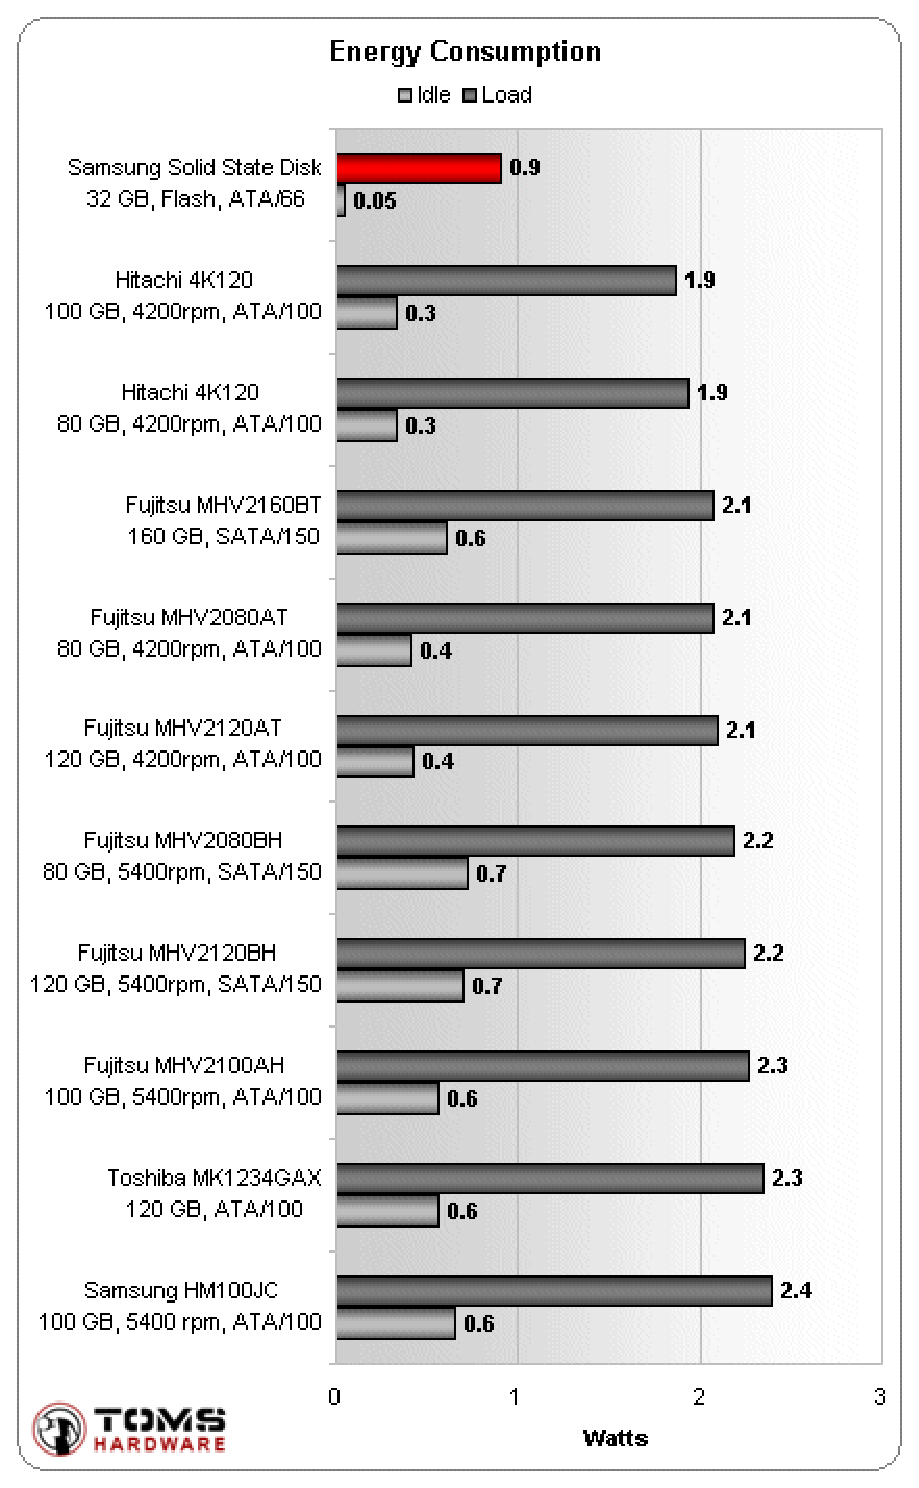
\includegraphics[scale=0.6]{graphics/power_consumption_harddrive}
                    \caption{Power Consumption for Hard-drives}
                    \label{fig:power_consumption_harddrive}
                \end{figure}
            \paragraph*{Chassis} Concerning power supply, fans or other PC components not belonging to the main parts, it is necessary to require quality other than price. Heating and cooling are really where the power consumption goes. Most computers only make up a fairly small percentage of your electrical bill. One should never underestimate the efficiency of the power supply, because most low quality ones are only about 45-55\% efficient, whereas it is possible to achieve more than 80\%.
            \paragraph*{Monitor Type} As shown by Table~\ref{tab:energy_used_monitor}\footnote{\url{http://michaelbluejay.com/electricity/computers.html}}, flat panel liquid crystal display (LCD) monitors power consumption equals to half the power of conventional CRT monitors. LCD monitors also dissipate less heat, which helps to reduce air conditioning costs. Another interesting point is that either LCD or CRT monitors consume the same amount of energy with or without screensavers. As LCD monitors do not consume much energy when turned off, that would be the best solution for idle computers.
                \begin{table}[h!tb]
                    \centering
                    \begin{tabular}{|c|c|}
                    \hline
                    \multicolumn{ 2}{|c|}{{\bf Monitors}} \tnhl
                    Typical 17" CRT &   80 watts \tnhl
                    Typical 17" LCD &   35 watts \tnhl
                    Apple MS 17" CRT$^a$ &   63 watts \tnhl
                    Apple MS 17" CRT$^b$ &   54 watts \tnhl
                    Screen saver$^c$ & same as above \tnhl
                    Sleeping monitor$^d$ & 0-15 watts \tnhl
                    Monitor turned off at switch & 0-10 watts \tnhl
                    \end{tabular}  \linebreak
                    $^a$ mostly white (blank IE window) \linebreak
                    $^b$ mostly black (black Windows desktop with just a few icons)\linebreak
                    $^c$ any image on screen\linebreak
                    $^d$ dark screen
                    \captionof{table}{Energy used by Monitors} 
                    \label{tab:energy_used_monitor}
                \end{table}

    \subsection{Policies / Tools / Labels} \label{sec2:policies_tools_labels}
        The amount of saved energy depends also on policies that regard technology acquisition and IT management, which may be enforced by a variety of specialized tools. Examples of policies that regard equipment acquisition are: the acquisition of new computers or components labeled as green by the manufacturer, purchase of computers with multi-core processors and even to discourage the purchase of specific kinds of hardware such as dual or large monitors and graphic cards. Another kind of policy relates to the management of the machines. One example of the latter is to turn off workstations or servers if they are going to be unused for a long time. This kind of measure is particularly efficient as a computer in idle mode uses 20 to 50 times the power of a computer in standby mode\footnote{\url{http://www.cosn.org/Initiatives/GreenComputing/EnergyUse/tabid/4515/Default.aspx}}.
        
    \begin{table}[h!tb]
        \centering
        \begin{tabular}{|c|c|}
        \hline
        \multicolumn{ 2}{|c|}{{\bf Computers}} \tnhl
        Desktop Computer & 60-250 watts \tnhl
        On screen Saver$^a$ & 60-250 watts \tnhl
        Sleep / Standby & 1-6 watts \tnhl
        Laptop & 15-45 watts \tnhl
        \end{tabular}\linebreak
        $^a$ no difference
        \captionof{table}{Energy used by a standard computer} 
        \label{tab:energy_used_computer}
    \end{table}

        The tools that automate these methods have as their main feature the possibility to let computers in a network in standby mode or even to turn them off after a long period of no utilization. In addition, the shared usage of networked pieces of hardware can be an effective way to achieve energy savings. Networked systems allow several nearby users to share a single printer, which generally generates savings in both equipment cost and energy if compared with each computer having a dedicated printer. Above that, choosing multifunction devices (MFD) that encapsulates in one machine the functionality of many others. In addition to saving space and materials, these multifunctionals save energy if compared to several different machines working in parallel. The Table~\ref{tab:energy_recommendation_efficient_printer}\footnote{\url{http://www1.eere.energy.gov/femp/procurement/eep_printer.html}} describes the power consumption in standby mode that an energy-efficient networked printer should have in relation to the printer type and to the number of pages it prints per minute. 
        
        \begin{table}[h!tb]
        \centering
            \begin{tabular}{|r|c|c|}
            \hline
            \multicolumn{ 3}{|c|}{{\bf Efficiency Recommendation}} \tnhl
            \multicolumn{ 1}{|c|}{Printer Speed} & \multicolumn{ 2}{|c|}{Recommended ``Sleep'' Mode$^a$} \tnhl
            \multicolumn{ 1}{|c|}{} & Laser B/W + All Ink jet$^b$ & Laser Color$^c$ \tnhl
            $\geq$10 pages/min & 10 watts or less & 35 watts or less \tnhl
            11-20 pages/min & 20 watts or less & 45 watts or less \tnhl
            21-30 pages/min & 30 watts or less & 70 watts or less \tnhl
            31-44 pages/min & 40 watts or less & 70 watts or less \tnhl
            $>$44 pages/min & 75 watts or less & 70 watts or less \tnhl
            \end{tabular}\linebreak            
            $^a$ ``Sleep'' mode is a low-power standby condition, it restores automatically with a print request.\linebreak
            $^b$ Includes both black-ink and color ink jets, and printer/fax combinations.\linebreak
            $^c$ Also includes LED and thermal transfer color printers.
            \captionof{table}{Energy Recommendation to an Energy-Efficient Printer} 
            \label{tab:energy_recommendation_efficient_printer}
        \end{table}
        
        One last kind of policy is to favor the acquisition of eco-labeled products. An eco-label is given to products that comply with some energy efficiency specifications. The most famous of these labels is the ENERGY STAR$^{\textcircled {\scriptsize R}}$, which is an energy efficiency program sponsored by the U.S. Environmental Protection Agency. For example, An ENERGY STAR$^{\textcircled {\scriptsize R}}$ qualified computer is possible to use up to 70\% less electricity than computers without enabled power management features.
            
        \subsection{Thin Client Architectures} \label{sec2:thin_clients}
            According to \emph{Wikipedia}, in 2009, ``a thin client is a client computer or client software in client-server architecture networks which depends primarily on the central server for processing activities, and mainly focuses on conveying input and output between the user and the remote server''. This is very well connected to both ideas of cloud computing and Green ICT and it is possible to subdivide in three categories for comparison against standard the PC architecture: Performance, Power Consumption and Hardware Savings and they are going to be exploited in the following subsections.
            
            \subsubsection*{PC vs. Thin Client: Performance}
                In order to analyze and give a comparison base of the performance between standard PCs and two types of thin clients, a set of tests were executed. The variable that was the number of active clients on a network, each running the same typical office applications tasks. The following client platforms were considered in this study:
                \begin{itemize}
                    \item PC: OptiPlex 210L PCs, basic managed PC desktops running Windows XP Professional;
                    \item Sun thin client: Sun Ray 2 running Sun Ray proprietary software;
                    \item Wyse thin client: Wyse Winterm 5150SE, Linux-based thin clients running Wyse Linux V6.
                \end{itemize}
                Each network used a standard file server, an HP ProLiant DL360 3.4MHz with and Intel Xeon processor and Microsoft Server 2003 Enterprise Edition. For test reasons, all the files that were manipulated by the PC were stored at the server. The tests are listed below:
                \begin{itemize}
                    \item Calculating subtotal in Microsoft Office Excel 2003 (Figure~\ref{fig:graphic_excel_test} and Table~\ref{tab:table_excel_test})
                    \item Compressing a PDF within Adobe Acrobat 7.0 Standard (Figure~\ref{fig:graphic_pdf_test} and Table~\ref{tab:table_pdf_test})
                \end{itemize}
                
                \begin{figure}[h!tb]
                    \centering
                    \resizebox{\textwidth}{!}{ % Fazendo a tabela caber no espaco da pagina
                    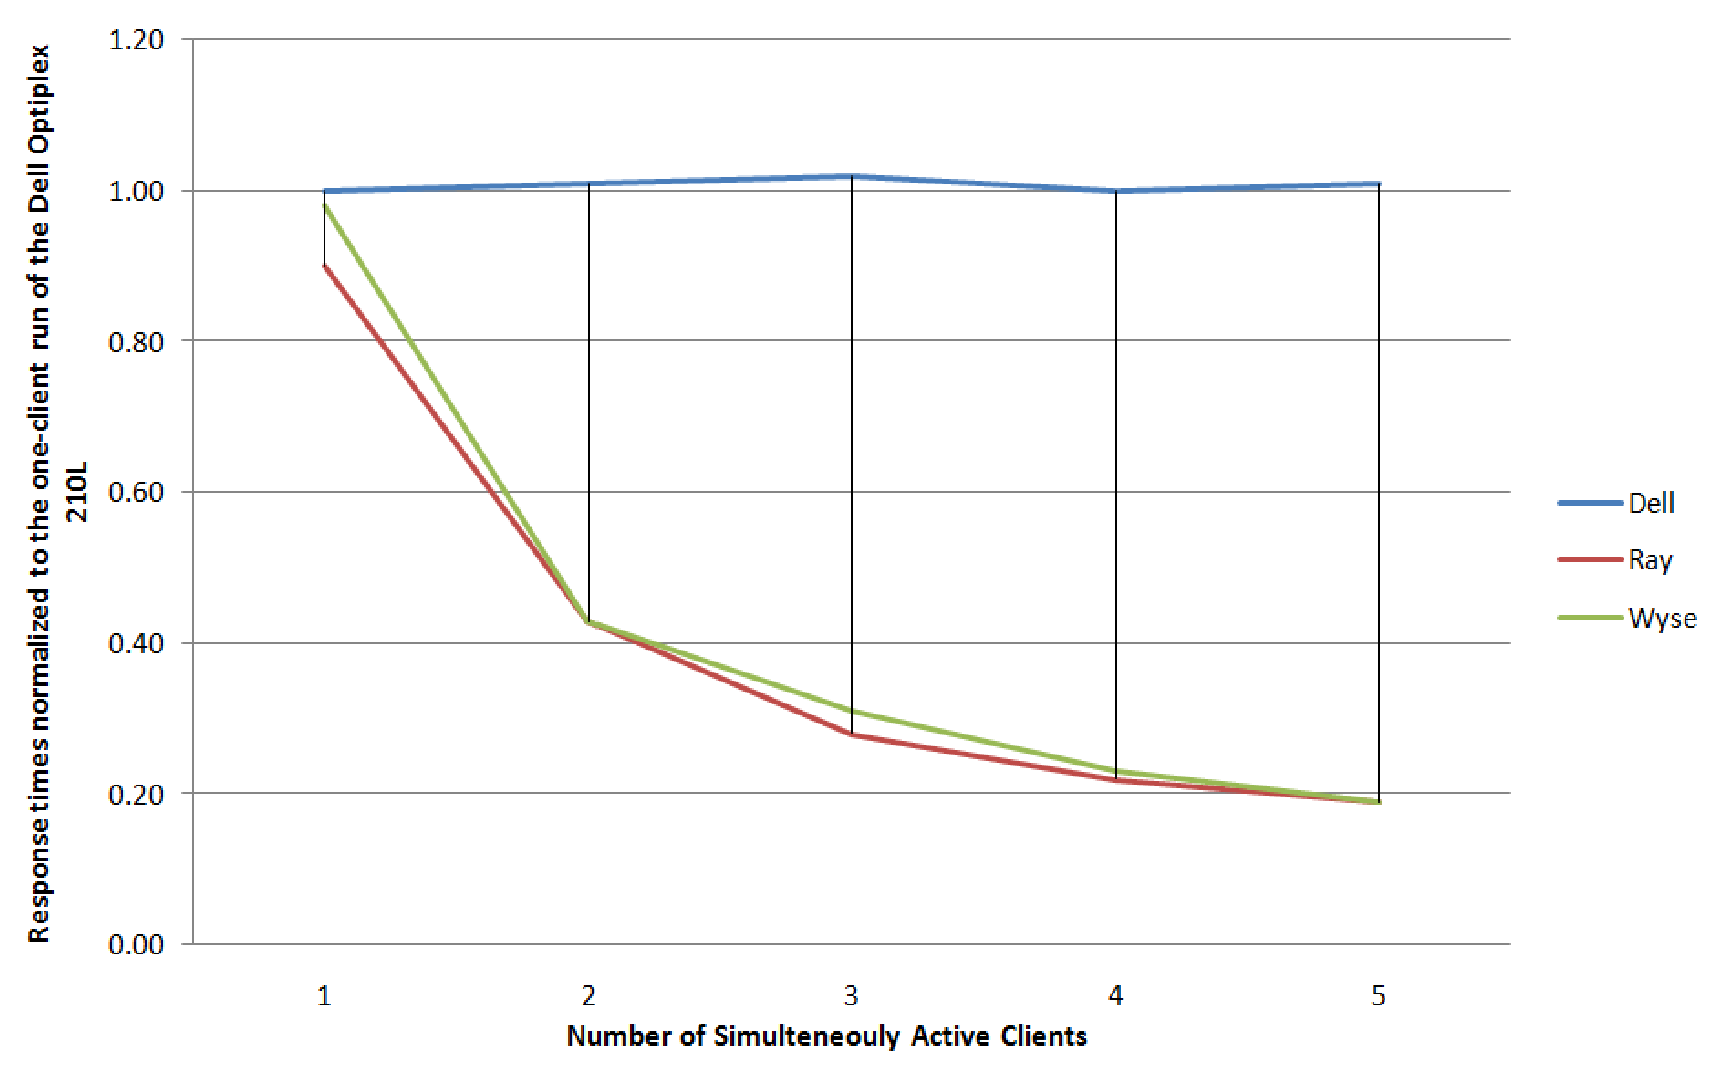
\includegraphics{graphics/graphic_excel_test}}
                    \caption{Normalized Excel Subtotals Task Response Times}
                    \label{fig:graphic_excel_test}
                \end{figure}
                \begin{table}[h!tb]
                    \centering
                    \begin{tabular}{|c|c|c|c|c|c|c|}
                    \hline
                    \multicolumn{ 3}{|c|}{Performance Results} &            & \multicolumn{ 3}{|c|}{Comparative Rating} \tnhl
                    PC solution & \multicolumn{ 2}{|c|}{Thin-client solutions} & Number of   & PC solution & \multicolumn{ 2}{|c|}{Thin-client solutions} \tnhl
                          Dell &        Sun &       Wyse & concurrent &       Dell &        Sun &       Wyse \tn

                      OptiPlex &        Ray &    Winterm &     active &   OptiPlex &        Ray &    Winterm \tn

                          210L &          2 &     5150SE &    clients &       210L &          2 &     5150SE \tnhl
                          12.9 &       13.2 &       13.1 &          1 &       1.00 &       0.90 &       0.98 \tnhl
                          12.8 &       30.2 &       29.7 &          2 &       1.01 &       0.43 &       0.43 \tnhl
                          12.7 &       45.5 &       41.9 &          3 &       1.02 &       0.28 &       0.31 \tnhl
                          12.9 &       58.3 &       57.3 &          4 &       1.00 &       0.22 &       0.23 \tnhl
                          12.8 &       68.1 &       67.9 &          5 &       1.01 &       0.19 &       0.19 \tnhl
                    \end{tabular}  
                    \captionof{table}{Performance Results for Excel Subtotals Calculation} 
                    \label{tab:table_excel_test}
                \end{table}
                \begin{figure}[h!tb]
                    \centering
                    \resizebox{\textwidth}{!}{ % Fazendo a tabela caber no espaco da pagina
                    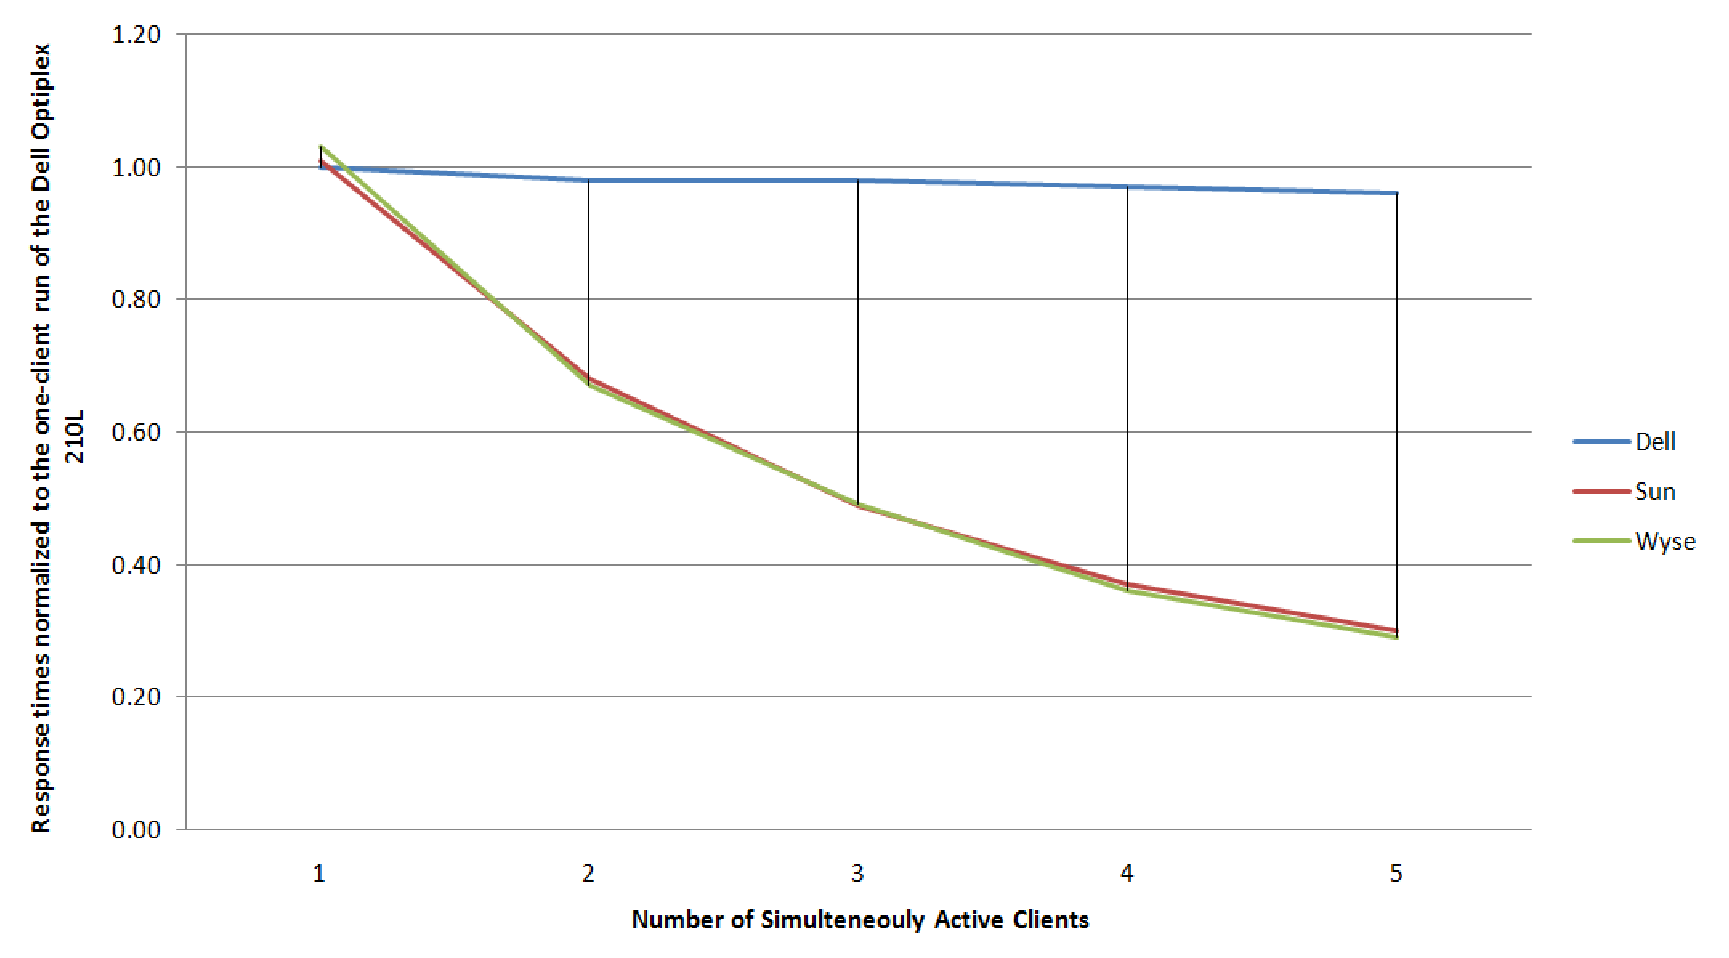
\includegraphics{graphics/graphic_pdf_test}}
                    \caption{Normalized PDF Subtotals Task Response Times}
                    \label{fig:graphic_pdf_test}
                \end{figure}
                \begin{table}[h!tb]
                    \centering
                    \begin{tabular}{|c|c|c|c|c|c|c|}
                    \hline
                    \multicolumn{ 3}{|c|}{Performance Results} &            & \multicolumn{ 3}{|c|}{Comparative Rating} \tnhl
                    PC solution & \multicolumn{ 2}{|c|}{Thin-client solutions} & Number of   & PC solution & \multicolumn{ 2}{|c|}{Thin-client solutions} \tnhl
                        Dell   &        Sun &       Wyse & concurrent &     Dell   &        Sun &       Wyse \tn

                      OptiPlex &        Ray &    Winterm &     active &   OptiPlex &        Ray &    Winterm \tn

                          210L &          2 &     5150SE &    clients &       210L &          2 &     5150SE \tnhl
                          16.1 &       16.0 &       15.6 &          1 &       1.00 &       1.01 &       1.03 \tnhl
                          16.4 &       23.8 &         24 &          2 &       0.98 &       0.68 &       0.67 \tnhl
                          16.5 &       33.0 &       33.1 &          3 &       0.98 &       0.49 &       0.49 \tnhl
                          16.6 &       43.7 &       44.3 &          4 &       0.97 &       0.37 &       0.36 \tnhl
                          16.7 &       54.0 &       55.1 &          5 &       0.96 &       0.30 &       0.29 \tnhl
                    \end{tabular}  
                    \captionof{table}{Performance Results for PDF Compression Subtotals Calculation}
                    \label{tab:table_pdf_test}
                \end{table}
                \pagebreak
            \subsubsection*{PC vs. Thin Client: Power Consumption}
                Supposing 30 thin users share a 400W server, the total power consumption will be 1300W - a yearly cost of \euro640.00. 30 PCs would consume 10000W instead - a yearly cost of \euro4900.00 (assuming the MWh cost is \euro80.00). The Table~\ref{tab:pc_thin_client_power_consumption} shows the power consumption of thin-client and PC.
                \begin{table}[h!tb]
                \centering
                    \begin{tabular}{|c|c|c|}
                    \hline
                         & {\bf Thin Client} &   {\bf PC} \tnhl
                    {\bf Weight} & 2.2 - 7.7 lbs & 22 - 33 lbs \tnhl
                    {\bf Volume} & 1.5 - 3 dm$^3$ & 30 - 35 dm$^3$ \tnhl
                    {\bf Packing material} & 2.2 - 4.4 lbs &   3 - 5 kg \tnhl
                    {\bf Power consumption\linebreak (including monitor)} & 20 - 50 watt & 300 - 400 watt \tnhl
                    {\bf Heat rejection} & 5 - 35 watt & 85 - 115 watt \tnhl
                    {\bf Noise level} & 0 dbA & 50 - 60 dbA \tnhl
                    \end{tabular}  
                    \captionof{table}{PC and thin client power consumption} 
                    \label{tab:pc_thin_client_power_consumption}
                \end{table}
                
            \subsubsection*{Hardware Savings}
                \paragraph*{Savings on client hardware} 
                    The economy brought by the substitution of PCs with thin clients was estimated around US\$ 208 per PC per year. The estimative considered the average prices of a PC, an adequate thin client and the PC upgrade costs every 3 years. If energy consumption is considered, the savings will be even greater.

                The following considerations were taken:
                \begin{itemize}
                    \item Thin client cost: US\$250.00 x PC cost: US\$750.00;
                    \item PC needs to be upgraded every 3 years and thin clients need to be replaced every 6 years.
                \end{itemize}
                Therefore, in a 6-year period US\$1500.00 will be spent on a PC against US\$250.00 that will be spent on a thin client.

            \paragraph*{Extra server hardware costs}
                Considering that:
                \begin{itemize}
                    \item On average 30 users will need a dual processor server with 4 GB of RAM and SCSI hard disks;
                    \item A brand new server should cost around US\$4,500.00 and will depreciate on average in 3 years.
                \end{itemize}
                For 60 users, the thin client solution should out-price the PC one by US\$11,300.00 per year, excluding the administration costs of both solutions.

        \subsection{Servers and Virtualization} \label{sec2:servers_virtualization}
                        
            \subsubsection*{Rack vs. Blade}
                According to Goldworm\cite{barbAnne07}, Blade servers are a package of ``ultra-high density components including servers, storage, and communications interfaces in a pre-wired chassis with shared components such as power, cooling, and networking. In contrast to the conventional \emph{horizontal} positioning within a rack (rack mounted servers), blades servers are typically (though not always) installed \emph{vertically} in a blade chassis, like books in a bookshelf''. This disposition of the blade servers along with their reduced dimension provide a high server density and thus of performance. For example, 60 blade servers such as the one depicted in Figure~\ref{fig:example_blade_server} can fit in the same physical space as 42 rack-mounted servers. A blade enclosure, which can hold from 8 to 24 \cite{Rehn08} blade servers, provides common services such as power supply, cooling and networking thus eliminating redundancies in each individual blade server. A standard rack can accommodate more than 250 blade servers against approximately 42 standard servers.
            \begin{figure}[h!tb]
                \centering
                \subfloat[IBM LS20]{
                    \label{fig:ibm_ls20_blade_server}
                    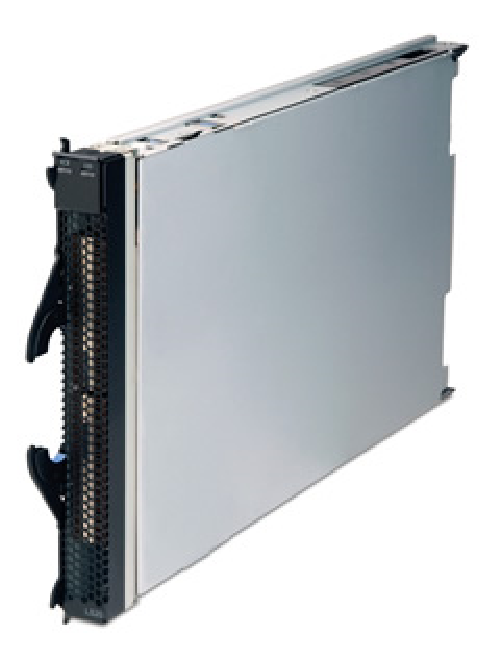
\includegraphics[width=0.3\textwidth]{graphics/ibm_ls20_blade_server}}
                \subfloat[Sun 6000 Series Blade Enclosure]{
                    \label{fig:sun_6000_blade_enclosure}
                    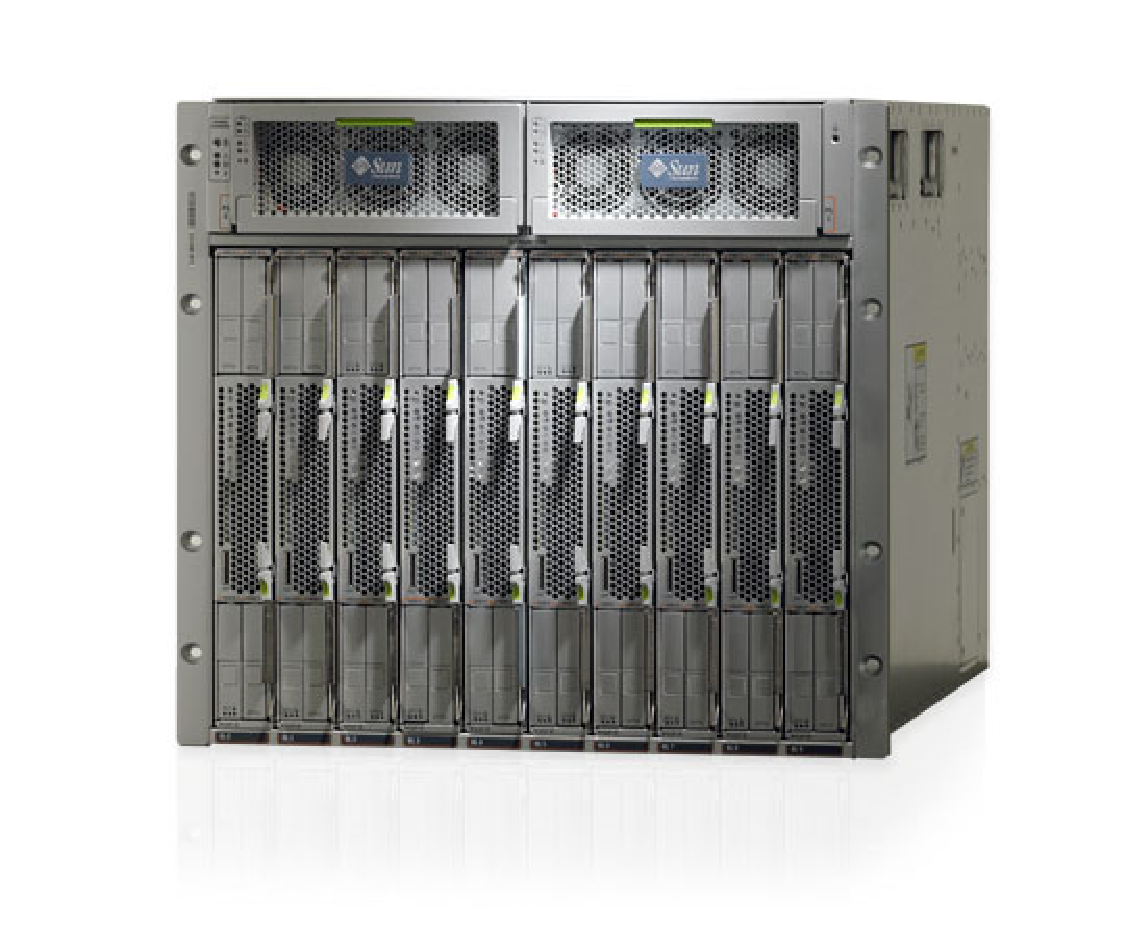
\includegraphics[width=0.3\textwidth]{graphics/sun_6000_blade_enclosure}}
                \subfloat[HP Intros Rack]{
                    \label{fig:hp_intros_blade_server_rack}
                    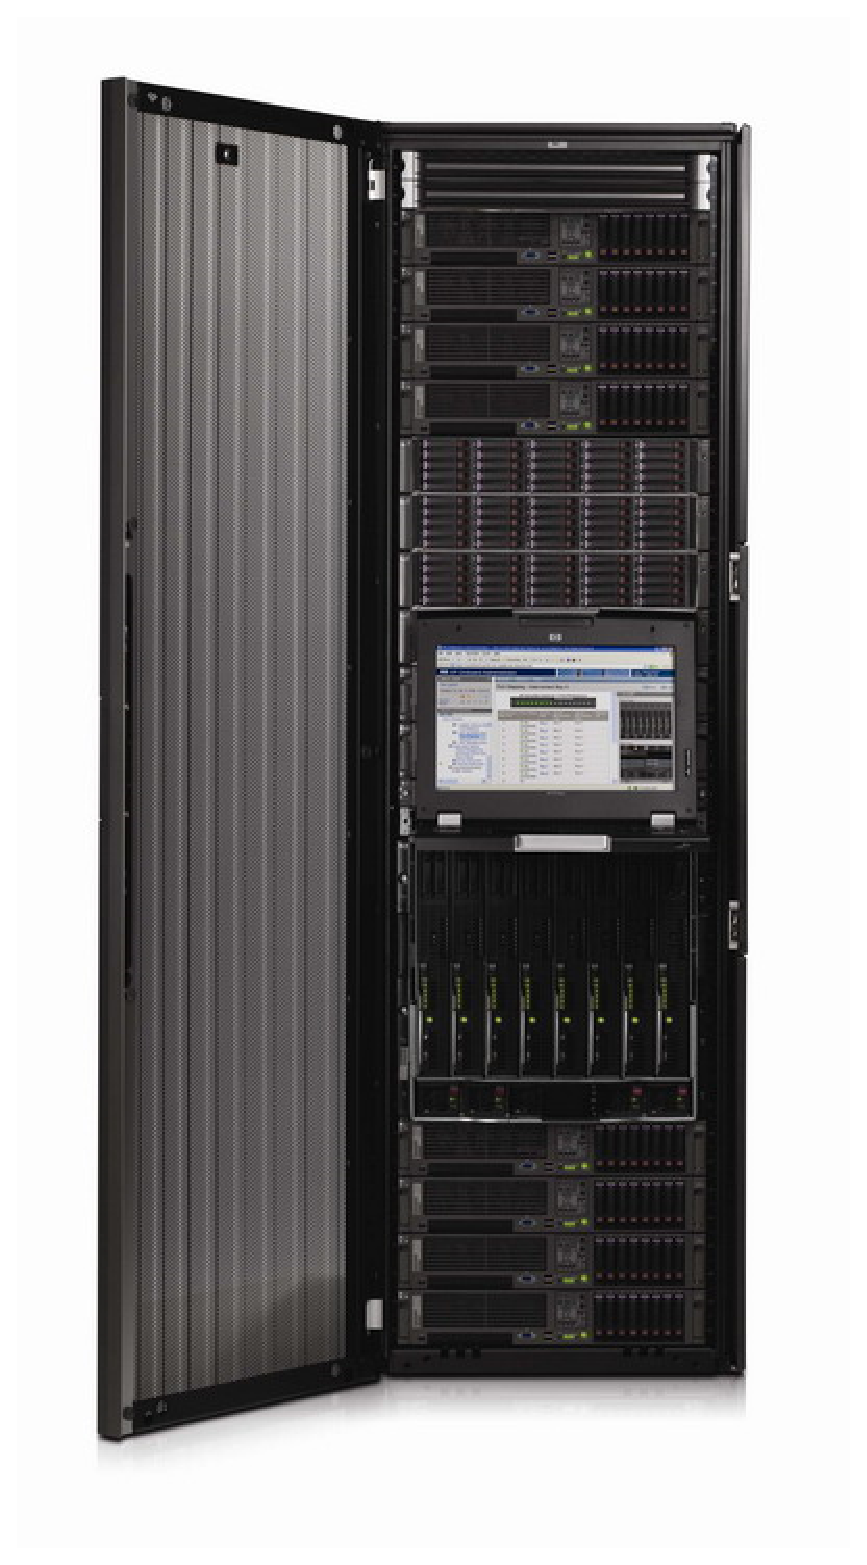
\includegraphics[width=0.3\textwidth]{graphics/hp_intros_blade_server_rack}}
                \caption{Examples of Blade Servers}
                \label{fig:example_blade_server}
            \end{figure}
            \begin{figure}[h!tb]
                \centering
                \subfloat[Chenbro 5U RM51924]{
                    \label{fig:chenbro_5urm51924}
                    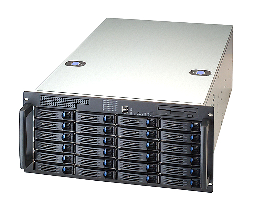
\includegraphics[width=0.3\textwidth]{graphics/chenbro_5U_RM51924}}
                \subfloat[Rack Server]{
                    \label{fig:rack_server}
                    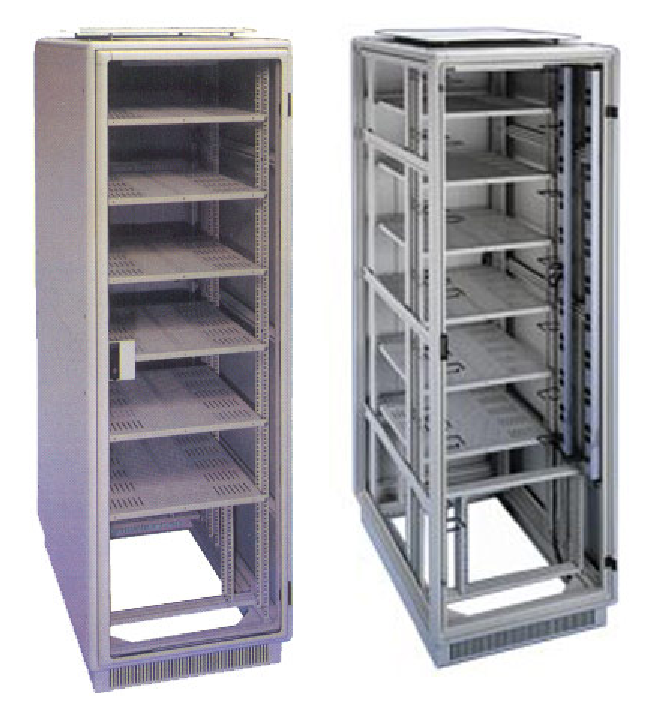
\includegraphics[width=0.3\textwidth]{graphics/rack_server}}
                \caption{Examples of Rack Servers}
                \label{fig:example_rack_server}
            \end{figure}
            In the Table~\ref{tab:power_consumption_several_servers}, a comparison is made between IBM HS21 blades and x3550 rack servers. The blades and rack servers have comparable performance.
            \begin{itemize}
                \item 2.0 GHz intel quad core;
                \item 8 GB DDR2 memory;
                \item Both in standard configuration, with no HDDs.
            \end{itemize}
            \begin{table}[h!tb]
                \centering
                \begin{tabular}{|c|c|c|c|}
                \hline
                \multicolumn{ 1}{|c|}{{\bf IBM server model}} & \multicolumn{ 1}{|c|}{{\bf Base Power}} & \multicolumn{ 1}{|c|}{{\bf kWh consumed}} & \multicolumn{ 1}{|c|}{{\bf Total cost }} \tn
                \multicolumn{ 1}{|c|}{{\bf }} & \multicolumn{ 1}{|c|}{{\bf Consumption}} & \multicolumn{ 1}{|c|}{{\bf over 5 years}} & \multicolumn{ 1}{|c|}{{\bf (\$0.03/kWh)}} \tn
                \multicolumn{ 1}{|c|}{{\bf }} & \multicolumn{ 1}{|c|}{{\bf }} & \multicolumn{ 1}{|c|}{{\bf }} & \multicolumn{ 1}{|c|}{{\bf over 5 years}} \tnhl
                BC-H Chassis, no blades & 0.510 kWh &     22,350 &  \$670.50  \tnhl
                BC-H HS21 blade & 0.318 kWh &     13,936 &  \$418.08  \tnhl
                x3550 server & 0.373 kWh &     16,346 &  \$490.39  \tnhl
                x3650 server & 0.455 kWh &     19,940 &  \$598.20  \tnhl
                BC-H chassis with 14 & 4.962 kWh &    217,455 & \$6,523.65  \tn
                HS21 blades &  &  &  \tnhl
                14 x3550 servers & 5.222 kWh &    228,849 & \$6,865.46 \tnhl
                14 x3650 servers & 6.370 kWh &    279,259 & \$8,374.80  \tnhl
                \end{tabular}  
                \captionof{table}{Power consumption for several servers, excluding cooling and redundancy}%XXX colocar referencia
                \label{tab:power_consumption_several_servers}
            \end{table}

            \begin{itemize}
                \item Space saving and efficiency - packing more computer power in a significantly smaller area;
                \item Consolidation of servers to improve and centralize management as well as utilization;
                \item Return on investment (ROI) and improved total cost of ownership (TOC) through increased hardware utilization and reduced operating expenses;
                \item More energy efficient, due to existence of centralized power supply, cooling and networking.
            \end{itemize}
            According to the figures, the choice of using a blade server provides roughly 5\% power saving over a similar rack-mount configuration. The main benefit brought by the use of blade servers, however, is the processing density, as a rack filled with blade servers may carry up to 50\% more servers than one with rackable servers. Other benefits are that blade servers are easier to service and reduce the number of power cables needed from as much as 80\% \cite{Hendenson07}. 
            
            In conclusion, blade servers do not provide much in terms of power saving but it greatly reduces the amount of space used in datacenters. However, the high power density might prove to be a problem to server farms in terms of overheating. Solutions to this problem are described in the section of Data Center Infrastructure.
            
            \subsubsection*{Virtualization}
                The overall goal of virtualization is to create a logical abstraction of physical assets. It allows multiple ``virtual'' servers to run on one physical server, thereby consolidating many physical servers into one. \emph{Wikipedia}, in 2009, defines virtualization as the following: ``Virtualization is the process of presenting a logical grouping or subset of computing resources so that they can be accessed in ways that give benefits over the original configuration. This new virtual \emph{view} of the resources is not restricted by the implementation, geographic location or the physical configuration of underlying resources.''. Virtualization can improve efficiency and availability of resources and applications in the organization and according to \emph{Vmware}, the choice of virtualized servers over the standard nonvirtualized configuration makes possible to save 50-70\% overall IT costs. Apart from the reduction of costs, virtualization may free up IT resources, provide better infrastructure optimization and utilization, increase availability and improve desktop management.
                
                Besides that, virtualization has made positive improvements to the environment issue. Gartner \cite{GartnetStamford07} estimates that 1.2 million workloads run in virtual machines, which represents an annual aggregate power savings of about 8.5 billion kWh - more electricity than is consumed annually in all of New England for heating, ventilation and cooling. While this is a good start, there are plenty of opportunities for saving even more energy and money. Analyst firm IDC \cite{IDCDoc07} states that the un-utilized server capacity equates to approximately:
                \begin{itemize}
                    \item in term of equipment and energy costs : US\$140 billion annually
                    \item in terms of hardware costs : 3 years supply of hardware
                    \item in terms of computing power : more than 20 million servers 
                \end{itemize}
                At the annual production rate of 4 tons of carbon dioxide (CO$_{2}$) per server, these un-utilized servers produce a total of more than 80 million tons of CO$_{2}$ per year. This is more than is emitted from the country of Thailand and more than half of all countries in South America. From the organizational point of view these data suggests that virtualization is a good improvement to the data center, saving not only space provided to the servers but also saving energy by reducing the idle time of the servers and augmenting their workload. It is also important to state that, by providing a virtualized solution, the number and variety of available applications can be increased.
                
                There are two kinds of virtualization that may be used in a data center: storage and computing virtualization. Storage-area networks (SAN) may be implemented to present several different physical storage racks as a single virtual storage pool \cite{Antonopoulos05}. On the other hand, computing virtualization can be implemented in two ways. The first case is when a single physical server can offer multiple virtual servers, each with its own OS. Another option is to consolidate multiple physical servers into a cluster that acts as a single server. There are cross-platform server virtualization softwares available which allows data center managers to cluster and partition servers.
                \begin{figure}[h!tb]
                    \centering
                    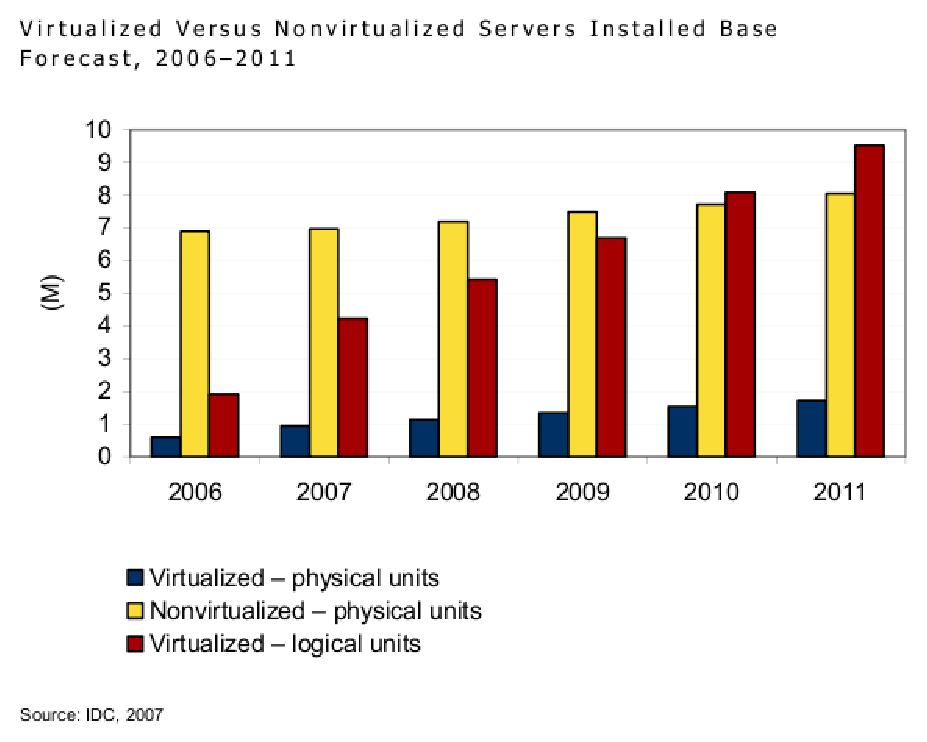
\includegraphics{graphics/installed_base_virtualized_servers}
                    \caption{Installed Base of Virtualized and Non-Virtualized Servers}
                    \label{fig:installed_base_virtualized_servers}
                \end{figure}
                
                According to the Figure~\ref{fig:installed_base_virtualized_servers} there is a trend indicating an increasing number of virtualized units over time along a forecast that by the end of 2009 the number of virtualized servers will be greater than non-virtualized ones. Logical units represent virtualized storage while physical units represent the use of non-virtualized storage. As shown in the Figure~\ref{fig:illustration_virtualization_to_physical_server}, virtualization tools such as VMware allow one physical server to act as a number of logical servers. VMware also provides a benchmark tool called VMmark\footnote{\url{http://www.vmware.com/products/vmmark/}} along with a set of test results in \cite{Makhija06} for a configuration that includes a mail server, a java server, a standby server, a web server, a database server and a file server.
                \begin{figure}[h!tb]
                    \centering
                    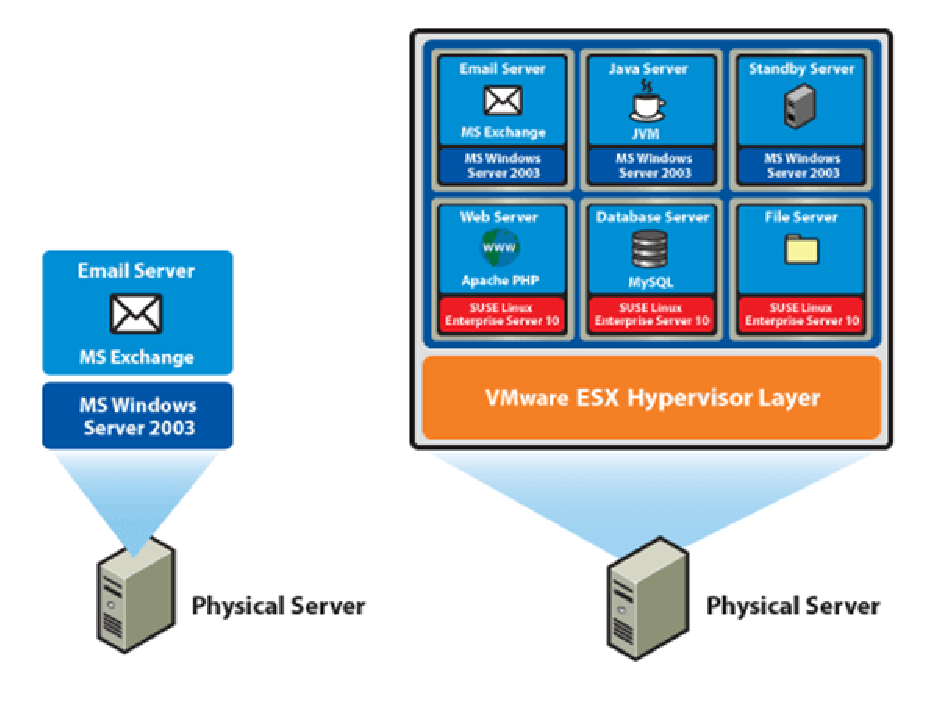
\includegraphics[scale=0.7]{graphics/illustration_virtualization_to_physical_server}
                    \caption{Illustration of Virtualization Applied to a Physical Server}
                    \label{fig:illustration_virtualization_to_physical_server}
                \end{figure}
                
                Coming along with the virtualization trend are high-throughput and eco-responsible processors such as the Sun's UltraSPARC T1 processor \cite{Hetherington05}, which support up to 128 virtualized systems in a single server and gives one of the best performance per watt of the available processors. As shown in the Table~\ref{tab:performance_power_dissipation_several_processors}\footnote{\url{http://www.anandtech.com/cpuchipsets/showdoc.aspx?i=2657&p=4}}, with relation to the UltraSPARC CPU the only comparable performance was met by the POWER5+ processor, which in average dissipates 4.5 times as much as the earlier.
                \begin{table}[h!tb]
                    \centering
                    \begin{tabular}{|c|c|c|c|c|c|c|}
                    \hline
                          &            & {\bf Power}       &                & {\bf Number}  &           &  \tn
                        &            & {\bf Dissipation} &                & {\bf of}      &           &  \tn
                        &            & {\bf CPUs}        & {\bf Number}   & {\bf Active}  & {\bf Score}   & {\bf Score} \tn
                  {\bf System} & {\bf CPU} & {\bf (Estimated)} & {\bf of cores} & {\bf Threads} & {\bf (bops)} & {\bf (\%)} \tnhl
                    Sun Fire  &  1x 1.2GHz &    72-79 W &          8 &         32 &     63.378 &      160\% \tn
                    T2000 & UltraSPARC T1 &            &            &            &            &            \tnhl
                    Sun Fire  &  2x 2.4GHz &  150-180 W &          4 &          4 &     45.124 &      114\% \tn
                    X4200 & DC Opteron &            &            &            &            &            \tnhl
                    IBM &  2x 1.9GHz &  320-360 W &          4 &          8 &     61.789 &      156\% \tn
                    p5 550 &    POWER5+ &            &            &            &            &            \tnhl
                    IBM 346 & 2x 2.8GHz  &  270-300 W &          4 &          8 &     39.585 &      100\% \tn
                    xSeries &    DC Xeon &            &            &            &            &            \tnhl
                    \end{tabular}
                    \captionof{table}{Performance and Power Dissipation for Several Processors by the Specjbb2005 Java Benchmark}
                    \label{tab:performance_power_dissipation_several_processors}
                \end{table}
                
        \subsection{Data Storage} \label{sec2:data_storage}
            There are currently three main technologies to store data: hard disks, tape drives and flash-based storage. This session will cover the first two, as they are the predominant technologies in datacenters. At the end of the session a comparison will be made between hard and tape drives.
            
            \subsubsection*{Tape Drives}
                A tape drive is a data storage device that reads and writes data stored on a magnetic tape. Its main use is as archival storage of data stored in hard drives. It is typically used for archival storage of data stored on hard drives. 
Tape media generally has a favorable unit cost, long archival stability and low energy consumption per MB of data stored to compensate for their slow seek times. Despite the slow seek time, tape drives can stream data to tape as quickly as hard drives. For example, modern LTO drives can reach continuous data transfer rates of up to 80MB/s, which is as fast as most 10,000rpm hard disks, according to \emph{Wikipedia, 2008}. Tape drives can range in capacity from a few megabytes to hundreds of gigabytes. Data can be compressed as to maximize the capacity usage. In this case the compression rate is of usually 2:1. A set of tables related to tape drives can be found in Appendix~\ref{app:comparison_tape_drives}
            
            \subsubsection*{Disk Arrays}
                Disk array refers to a linked group of one or more physical independent hard disks constituting a larger, high-performance system. They are usually implemented using RAID technology, which can provide component redundancy and high throughputs.
        
            \subsubsection*{Comparison between Tape Drives and Disk Arrays}
                Supposing a 995 TB database consisting of:
                \begin{itemize}
                	\item Storage base (frequently used data)
                	\item Backup cache (13 weeks)
                	\item Backup archive (1 year backup)
                \end{itemize}
                A solution consisting exclusively of disk arrays would require four 32-drawer disk array systems of 245 TB each. In order to ensure reliability and recoverability, a RAID5 format with two RAID5 arrays assigned to each drawer has been assumed. The total equipment cost is estimated on US\$10.57M \cite{Reine08} and according to the table~\ref{tab:tape_drive_power_costs} the disk array solution consumes 98KWh per TB per year.
                \begin{table}[h!tb]
                \centering 
                \resizebox{\textwidth}{!}{ % Fazendo a tabela caber no espaco da pagina
                \begin{tabular}{|c|c|c|c|c|c|c|c|c|}
                \hline
                & & {\bf Standby} & {\bf Per} & {\bf Number} & {\bf Total} & {\bf Power} &  & {\bf Annual} \tn
                & {\bf Processor} & {\bf Power} & {\bf SATA} & {\bf of SATA} & {\bf Array} &  {\bf Per} & {\bf Annual} & {\bf Cost} \tn
                {\bf Power} & {\bf Chassis} & {\bf Supply} & {\bf Drawer} & {\bf Drawers} & {\bf Power} &  {\bf Day} & {\bf Power} & US\$0.12/kWh \tnhl
                {\bf Typical} &  430 W/h &  34 W/h &  325 W/h &   32 &  11 kW/h & 264 kWh & 96,360 kWh & 11,563 \tnhl
                {\bf Maximum} &  800 W/h &  300 W/h &  425 W/h &   32 &  15 kW/h & 360 kWh & 131,400 kWh &  15,768 \tnhl
                \end{tabular}}
                \captionof{table}{Tape Drive Power Costs}%XXX verificar nome da tabela
                \label{tab:tape_drive_power_costs} %XXX verificar nome da tabela
                \end{table}
                With a native capacity of 800GB and throughput of 120 MB/sec, an LTO 4 drive has a compressed capability to write at 240 MB/sec, or 864 GB/hour. Supposing the same database is to be entirely stored at this drive, the equipment cost would be of US\$233,878.00 with an annual energy cost of US\$599.00.The tape solution will consume 1150 kWh in 1 year or 1,16kWh per TB per year.
                \begin{table}[h!tb]
                \centering 
                \resizebox{\textwidth}{!}{ % Fazendo a tabela caber no espaco da pagina
                \begin{tabular}{|c|c|c|c|c|c|c|c|c|}\hline
                {\bf N$^o$ of  } & {\bf N$^o$ of } & {\bf Library } & {\bf Frame} & & {\bf Drive} &  &   &  \tn
                {\bf frames} & {\bf drives } & {\bf acquisition } & {\bf acquisition } & {\bf Cartridge } & {\bf acquisition } & {\bf Space} & {\bf Energy} & {\bf Total} \tn
                {\bf acquired} & {\bf acquired} & {\bf cost} & {\bf cost} & {\bf cost} & {\bf cost} & {\bf cost} & {\bf cost} & {\bf cost} \tnhl
                1 &    2 &    76,000 &    30,000 &   82,278 &   45,600 &   68,850 &   599 &    303,327 \tnhl
                \end{tabular}}
                \captionof{table}{Disk Array Power Costs}%XXX verificar nome da tabela
                \label{tab:disk_array_power_costs} %XXX verificar nome da tabela
                \end{table}
                In overall, for the 995 TB database the following conclusions can be drawn:
                \begin{itemize}
	                \item Disk arrays consume 84 times as much as tape drives, per TB stored
	                \item The disk array solution costs 35 times as much as the tape drive solution
                \end{itemize}
                Although the cost difference between of both solutions may be high, performance should be also considered in the comparison. In that case, an adequate proportion between disk array and tape storage must be drawn according to the frequency of backup access.

        \subsection{Power Architectures} \label{sec2:power_architectures}
            \subsubsection*{Conventional AC Architecture}
                \begin{figure}[h!tb]
                    \centering
                    \resizebox{\textwidth}{!}{ % Fazendo a tabela caber no espaco da pagina
                    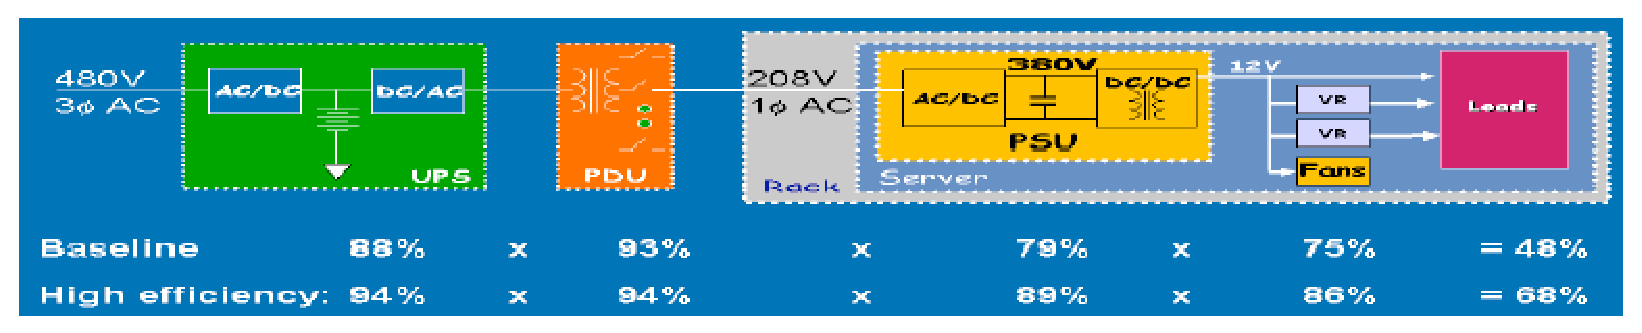
\includegraphics{graphics/conventional_ac_efficiency}}
                    \caption{Conventional AC architecture efficiency}
                    \label{fig:conventional_ac_efficiency}
                \end{figure}
                In this configuration (Figure~\ref{fig:conventional_ac_efficiency}) the following transformations take place:
                \begin{itemize}
	                \item PDU steps down the voltage from 480VAC to 208VAC;
                    \item Power Supply Unit (PSU) converts 208VAC to 380VDC;
                    \item Final component distribution at 12VDC.
                \end{itemize}
                The efficiency is measured for both conventional (baseline) and high efficiency (best-in-class) equipments. The difference in efficiency between the two equipment choices is of 20\%.

            \subsubsection*{Rack-Level DC Architecture}
                \begin{figure}[h!tb]
                    \centering
                    \resizebox{\textwidth}{!}{ % Fazendo a tabela caber no espaco da pagina
                    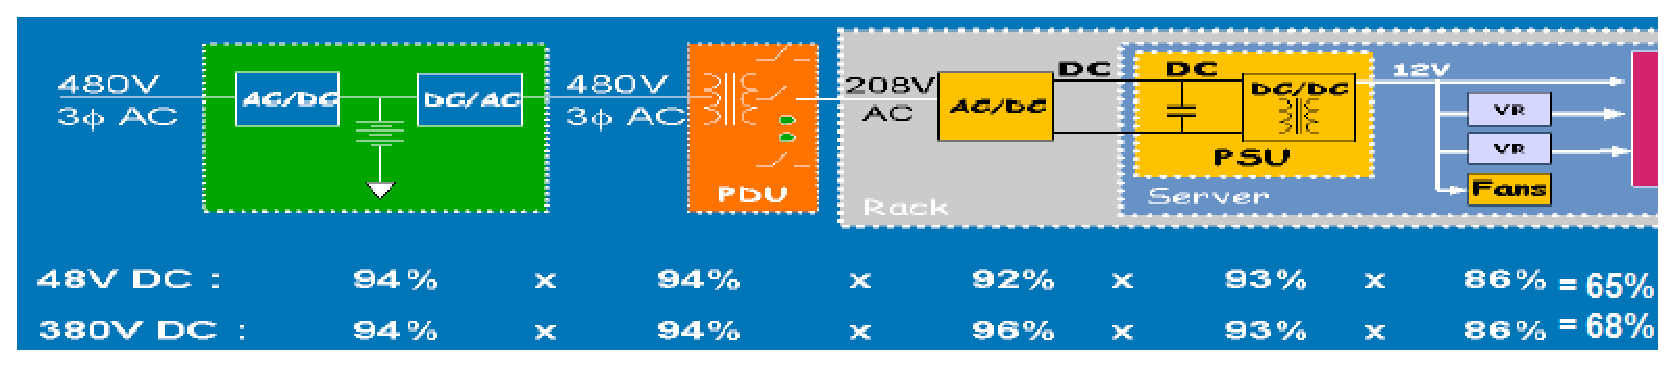
\includegraphics{graphics/rack_level_dc_efficiency}}
                    \caption{Rack-level DC architecture efficiency}
                    \label{fig:rack_level_dc_efficiency}
                \end{figure}
                On Figure~\ref{fig:rack_level_dc_efficiency}, it is possible to see that, after the PDU, an 208VAC to 48VDC/380VDC conversion is made in the rack. PSU and PDU are considered to be best-in-class, with high efficiency.

            \subsubsection*{Facility-level DC Architecture}
                \begin{figure}[h!tb]
                    \centering
                    \resizebox{\textwidth}{!}{ % Fazendo a tabela caber no espaco da pagina
                    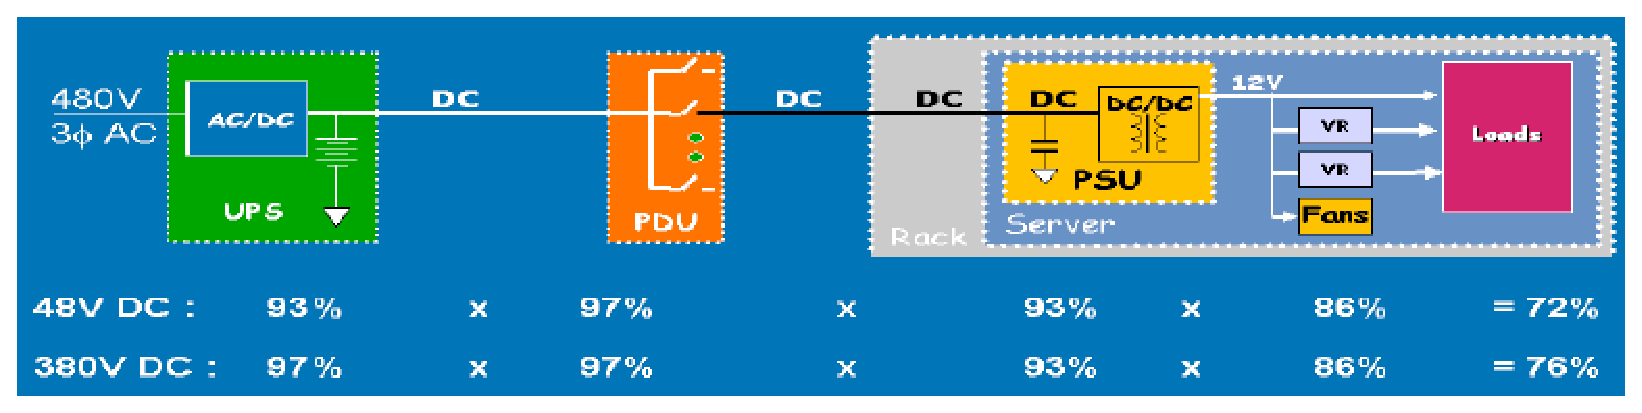
\includegraphics{graphics/facility_level_dc_efficiency}}
                    \caption{Facility-level DC architecture efficiency}
                    \label{fig:facility_level_dc_efficiency}
                \end{figure}
                In this configuration (Figure~\ref{fig:facility_level_dc_efficiency}), the DC-AC conversion in the UPS and the AC-DC conversion in the power supply are removed. It can be noted that the 480VAC-380VDC conversion in the UPS is more efficient than the 480VAC-48VDC conversion.
            
        \subsection{Data Center Infrastructure} \label{sec2:data_center_infrastructure}
            \subsubsection*{Water Cooling}
                The reasonable limit of rack power and cooling capacity for a conventional forced-air (HVAC) cooled data center is 8 kW per rack. For power densities approaching 15 kW per rack, the layout of the computing rooms and cooling facilities must be determined using specialized software (such as HP Static Smart Cooling). For racks requiring more than 15 kW, the latest cooling techniques use water (Figure~\ref{fig:power_consumption_number_servers_rack})~\cite{HPCooling07}.
                \begin{figure}[h!tb]
                    \centering
                    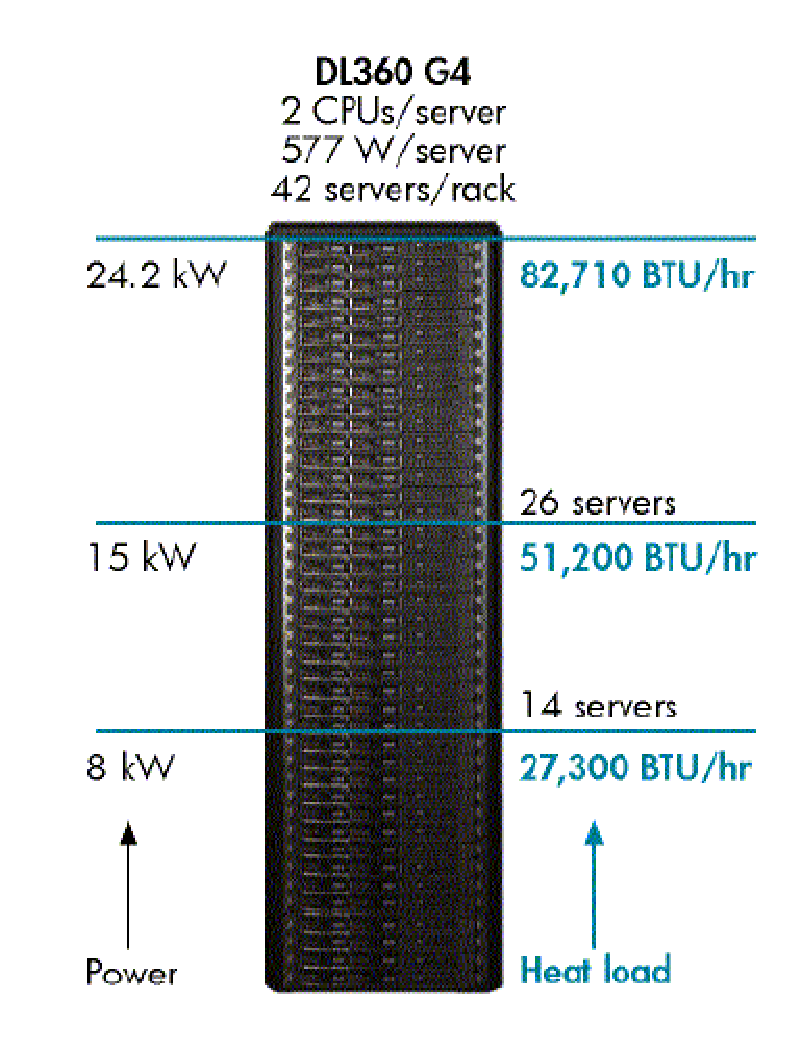
\includegraphics[scale=0.5]{graphics/power_consumption_number_servers_rack}
                    \caption{Power Consumption per Number of Servers in the Rack}
                    \label{fig:power_consumption_number_servers_rack}
                \end{figure}
                
                As shown in the figure~\ref{fig:footprint_reduction_for_35_heat_load}, the use of water cooling reduces in 50\% the equipment footprint, allowing greater server density. A 35 kW heat load dispersed among 4 racks could be concentrated in one single rack.
                
                \begin{figure}[h!tb]
                    \centering
                    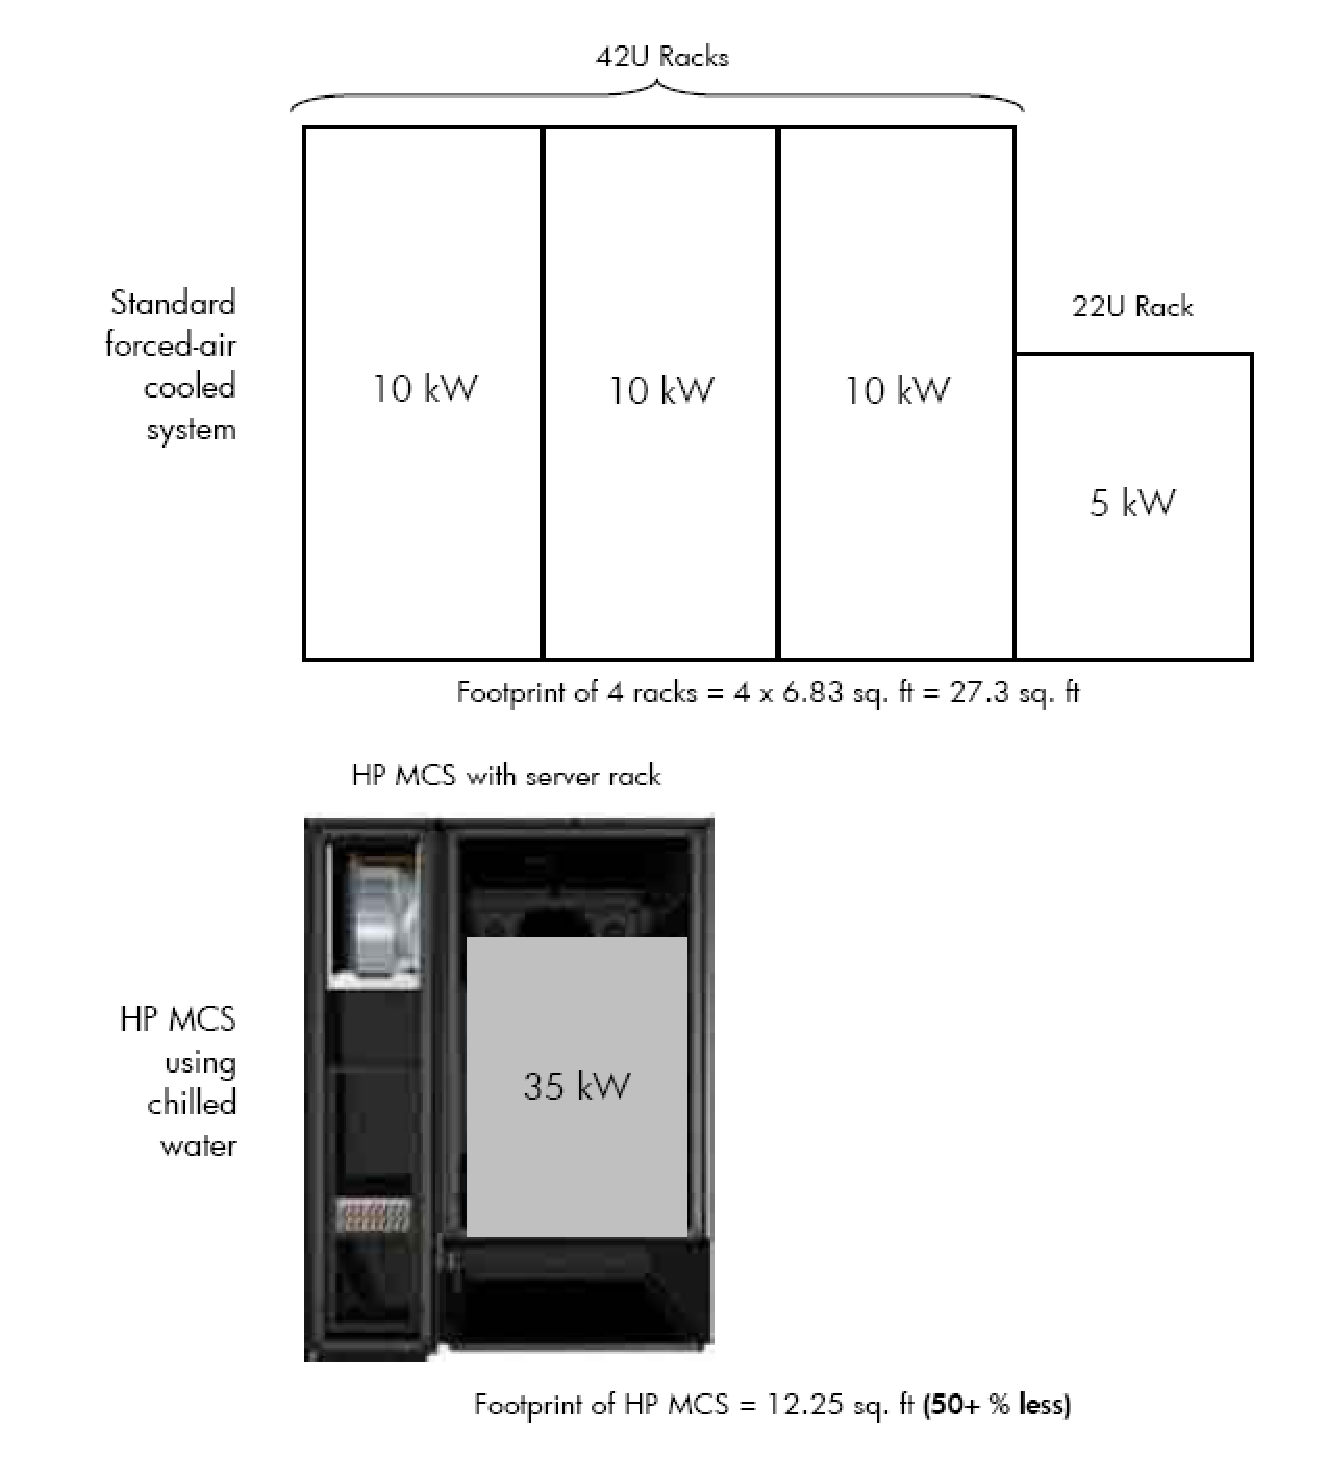
\includegraphics[scale=0.5]{graphics/footprint_reduction_for_35_heat_load}
                    \caption{Footprint Reduction for a 35 kW Heat Load}
                    \label{fig:footprint_reduction_for_35_heat_load}
                \end{figure}
                With relation to maintenance costs,
                \begin{figure}[h!tb]
                    \centering
                    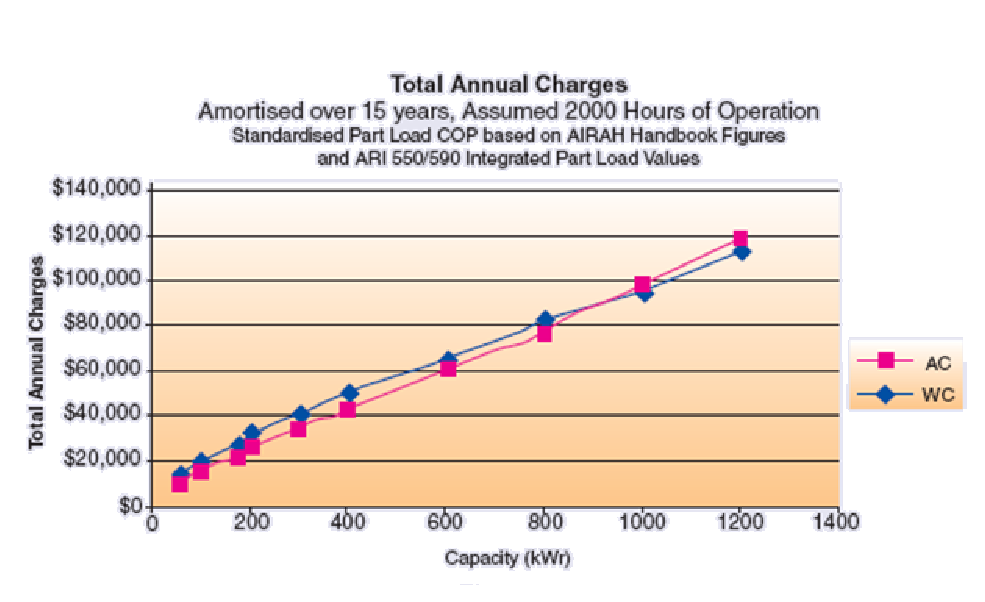
\includegraphics[scale=0.8]{graphics/economic_crossover_annualized}
                    \caption{Economic Cross-over of Annualized Charges Air-cooled to Water-cooled for 2000 Hours of Operations (in US \$)}
                    \label{fig:economic_crossover_annualized}
                \end{figure}
                \begin{figure}[h!tb]
                    \centering
                    \resizebox{\textwidth}{!}{ % Fazendo a tabela caber no espaco da pagina
                    \includegraphics[scale=0.5]{graphics/life_cycle_costs_water_cooled_air_cooled}}
                    \captionof{table}{Life Cycle Costs of Water-cooled and Air-cooled Solutions}
                    \label{tab:life_cycle_costs_water_cooled_air_cooled}
                \end{figure}
                The annual cost for water cooling and air cooling (including charges, maintenance, equipment) do not differ by a large amount as seen in Table~\ref{tab:life_cycle_costs_water_cooled_air_cooled} and Figure~\ref{fig:economic_crossover_annualized}. In this way, the main benefit brought by water cooling is the footprint reduction which can increase the server density in a data center.


%%%%%%%%%%%%%%%%%%%%%%%%%%%%%%%%%%%%%
%% Master Thesis - Computer Engineering
%% Copyright 2009 Ricardo Alexandre Fiorelli, Erick Poletto
%% This document is distributed by the terms of the license
%% included in the file LICENCE.
%%%%%%%%%%%%%%%%%%%%%%%%%%%%%%%%%%%%%

%%%%%%%%%%%%%%%%%%%%%%%%%%%%%%%%%%%%%
%% Third Chapter
%% Methodology
%%%%%%%%%%%%%%%%%%%%%%%%%%%%%%%%%%%%%

\chapter{Methodology} \label{chap3:methodology}

   This chapter will describe the steps taken to the end of constructing the components database and of validating the data contained in it.
These can be shortly described as follows:
    \begin{description}
        \item[Phase 0: Project definition -] As this work is part of a project aimed to create a methodology to implement a Green ICT strategy, this first phase consisted of the definition of the logical components of this project and of how the current work would collaborate to it;
        \item[Phase 1: Analysis of Benchmarking Softwares -] A number of existing softwares were analysed and those that have proven to be more adequate were selected. A list of the analysed softwares can be found in Appendix~\ref{app:list_other_energy_management_tools};
        \item[Phase 2: Catalog -] The tools were used to obtain information about computer components that were later used to create a component database;
        \item[Phase 3: Database design and construction -] The database schema was designed and data began to be inserted into the relations;
        \item[Phase 4: Analysis -] The validity of the stored data was tested with the help of direct measurements.
    \end{description}


\section{Overview} \label{sec3:overview}
    The main and broader objective of the research that is being conducted is to develop a methodology to implement a green ICT strategy. Namely, the methodology would provide a set of tools to guide the hardware acquisition process in an organization either in terms of workstations or of datacenter equipment. The present work will contribute to this research by providing a component database with information related to hardware components, which will be used as one of the inputs of the methodology. This work was conducted in order to determine how much energy a computer's components, for instance, CPU, Memory and Hard Drives spend and also how much they would affect the cost of acquisition of new computers as a whole. This is calculable with information such as component performance, power consumption and price. The analysis was carried out with the help of specialized softwares that will be described in the following sections and also with analytical measures made with an energy measurement device. In the end the benchmarking measures obtained from these softwares were compared with both the measures obtained from the device and with information provided by the component datasheets. With the benchmarking software, more than 1000 components were categorized in a database, whose schema can be found in Figure~\ref{fig:database_schema}. Firstly, the SiSoft Sandra's database~\ref{sec3:sandra} was used to collect the components and separate them by categories, along with their benchmark related data. Secondly, WebSPHINX~\ref{sec3:websphinx} was used to create a collection of components and their respective MPNs. In the end, an energy measurement device~\ref{sec3:energy_measurement_instrument} was used for the comparison and validation of the results given by the other benchmarks and acquisition of new data. 
    Finally, these data were all linked in a database for later comparison. 

\section{Research Design} \label{sec3:research_design} 
    The experimental method of research was used in this study. Figure~\ref{fig:experimental_method_approach} draws the steps of the method. To define the experimental type of research, Bryman \cite{bryman89} states that ``the experimental design (\ldots) allows the causal hypothesis that underpins the question to be examined'', which means that this method is a systematic and scientific approach to research in which the researcher manipulates one or more variables, controlling and measuring any changes in other variables. The emphasis given is on the results and analysis of the benchmarks provided and their measures. It allows to verify the thesis on which this work is based by making use of empirical methods which in the case relates to the benchmarks used.
    \begin{figure}[htbp]
        \centering
            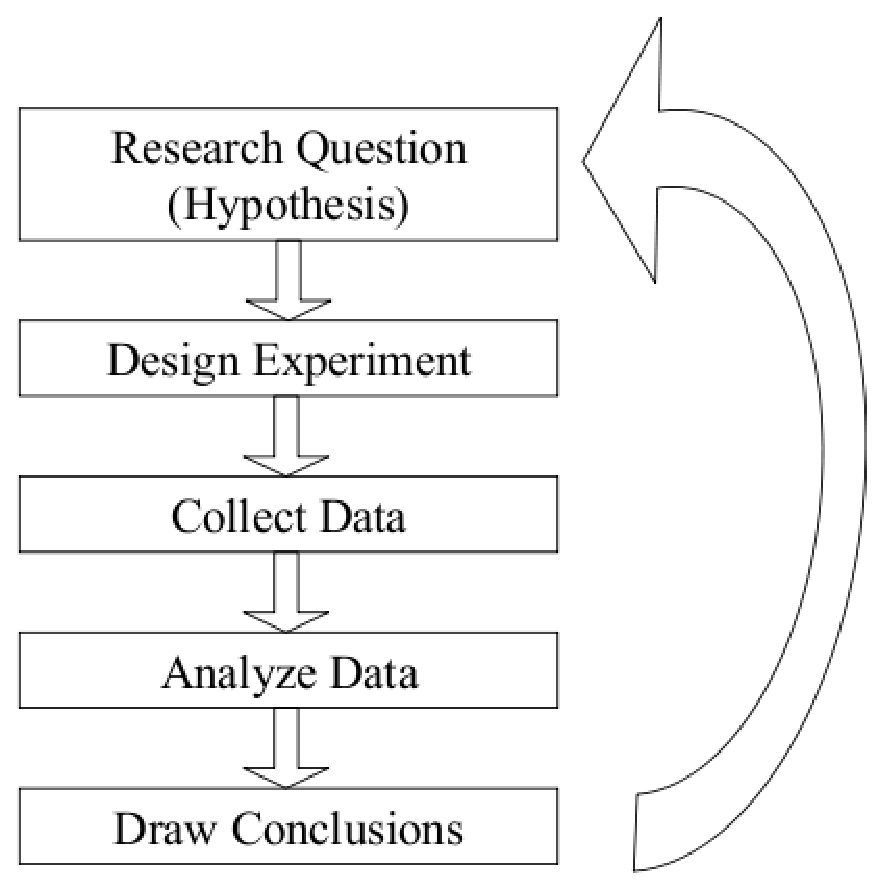
\includegraphics[scale=0.5]{graphics/experimental_method_approach}
            \caption{The Experimental Design Process}
            \label{fig:experimental_method_approach}
    \end{figure}

    % explicacao da figura
    %/********* Os proximos paragraphs foram criados para direcionar o pensamento e deve ser mantidos como comentario*******/
    %    \item[Universe o Study] (whether a tribe, or a village, or an urban areas, or a particular group, etc.) - no nosso caso, os componentes do computador e o data center
    The present study is meant to identify the power consumption of the computer components and to evaluate the accuracy of the obtained data through direct measurements. The quantitative method (direct measurements and benchmarking), other than the qualitative method, was employed in order to identify the more energy efficient components that may be used in green datacenters. Among all components, the ones included in the measurements are: Chipsets, Memory, Data Storage, Processor and the chassis (fan, power supply, etc).
    %    \item[Subject of Study] (whether it focuses on the whole society, or any specific institution or a part of it).
    The choice of analysing each component separately and also the whole computer power consumption was made in order to evaluate the behaviour of a machine configuration where a number of components have to interact and confront it to the expected behaviour of each component.
    %    \item[Relationship Between certain variables] (Formulating a Research Design but it is not obligatory to start with a Research Design).

    %    \item[Set of selected methods for obtain data] (whether participant observation, Interview, Questionnaire, or some other methods of data collection would be used).
    In order to obtain relevant data, three analysis' methods were used: empirical, benchmarking and research. For the empirical method, it was used an energy measurement device (section~\ref{sec3:energy_measurement_instrument}) that connected the electrical plug to the computer, and the measure was written in a spreadsheet~\ref{tab:toolino_table}. While doing this, the benchmarking tool (section~\ref{sec3:sandra}) was performed in the host computer in order to acquire measures in a set of different situations. The last method, the research, carried with the use of a web crawler called WebSPHINX, provided information about the price and the MPN of each component in the database. As each component has a unique MPN this made possible to uniquely identify each one of them, enabling thus the use of a normalized database over the identified components.

    %    \item[Analytical Categories] (by which the empirical data is subjected to analysis and interpretation).
    In a later stage, all the data acquired by the measurement approaches was separated by categories and components. The database generated is described and furtherly explained in the section~\ref{sec3:data_processing_analysis}.
    
\section{Energy Management and Benchmarking Tools} \label{sec3:energy_management_tools}
    In order to obtain relevant information about the data required for making the comparison between the components, some energy management and benchmarking tools were used.
    
    The softwares that used were selected over the other available ones for their superior evaluation on the following criteria:
\begin{description}
    \item[Size of Database] The database of components used by the software, in order to get a good result, should be considerably large;
    \item[Characteristics of Benchmarks] The benchmarks provided by the software should provide information about the energy consumed for each component;
    \item[Number of Benchmarks] The software should have a good variety of benchmarks;
    \item[Quality of Benchmarks] Although the number of benchmarks should be sufficient in number, the quality, precision and relevancy were also important in the decision method;
    \item[Ease of Use] In the sense that the software should provide an ambient of work that is both intuitive and user-friendly;
\end{description}
    
    The acquisition of data was made analysing the results of these benchmarks, making use of their database and system measurement capabilities.

    \subsection{SiSoftware SANDRA} \label{sec3:sandra}

    SiSoftware Sandra\footnote{The \textbf{S}ystem \textbf{AN}alyser, \textbf{D}iagnostic and \textbf{R}eporting \textbf{A}ssistant} is an information and diagnostic utility. It provides most of the information one need to know about their hardware, software and other devices whether hardware or software. SANDRA was the main software utilized to benchmark the data in this thesis work. It contains a vast database of components associated with both benchmark results and manufacturer specifications.
    
    This software gives the possibility of benchmarking computer devices at several levels of operation. For example, it can benchmark a processor and show its performance over several operational levels, from power saving to full workload. Moreover, it may monitor the performance in several levels, from the overall performance of a system to the performance of its components, including CPU, memory, hard disks, CD/DVD ROM, network adapters, etc. For that reason, it is considered one of the most complete benchmarking tools available. Besides the benchmarking, Sandra also provides hardware specifications for components such as the Motherboard, processor, disks, printers, etc. One last resource is the benchmarking of software performance, which is provided for key softwares (web browsers, e-mail program, etc.), OS information, processes, memory usage and more.
    
    The detailed list of modules utilized by SiSoftware Sandra can be found in Appendix~\ref{app:sandra_modules}.
    
    Furthermore, SiSoftware Sandra provides a catalogue of pricing, which, in addition to the power consumption and other important characteristics, enables the user to choose the best combination (which means the maximum performance/power ratio) of devices can be chosen to the server.
    
    \subsection{Energy Measurement Instrument} \label{sec3:energy_measurement_instrument}

        \begin{figure}[htbp]
            \centering
                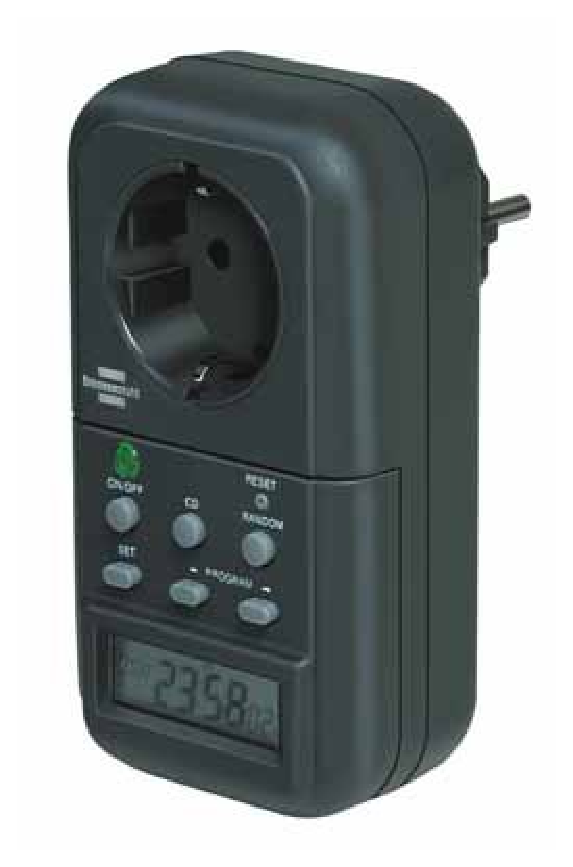
\includegraphics[scale=0.6]{graphics/energy_measurement_instrument}
                \caption{Energy Measurement Instrument}
                \label{fig:energy_measurement_instrument}
        \end{figure}
        The device, which can be seen on Figure~\ref{fig:energy_measurement_instrument}, was used for comparing and validating the results of the benchmarks given by Sandra. After the result of the benchmark was obtained from the SiSoftware Sandra, this equipment that was connected to the computer read how much energy it was consuming. The data from both sources were inserted in the database.
        
    \subsection{WebSPHINX - A Personal, Customized Web Crawler} \label{sec3:websphinx}
        WebSPHINX\footnote{Website-Specific Processors for HTML Information Extraction} is a Java class library used for web crawling. It provides a way to browse and process web pages automatically.
        
        This piece of software was used to determine the component's MPN code and also to create the pricing list, used in the database described in~\ref{sec4:analysis}.

        The target website used to obtain the information provided a specific search engine for each kind of component. The searches for each one of those used a base URL concatenated with a page number and the result pages were standardised and presented a list of components of a specific category (i.e. hard drives or processors) along their MPN number and suggested price. This made possible the automation of the search and the subsequent filtering of the desired information.\
        
        The individual components along with their MPN codes were inserted in the Device relation in the database while the pricing data were used in the Price relation.

    \subsection{CPU-Z} \label{sec3:cpu-z}
        CPU-Z detects information about the CPU, RAM Memory, motherboard, chip-set and more. That program was used to complete the database with missing information about the components.

        This software extracts system information such as name, number of cores, cache size and clock frequency for processors; mainboard model and chipset and size, bandwidth and type for main memory. This information is particularly useful when SiSoftware Sandra cannot identify a component or individuate its power consumption. The data obtained with the use of CPU-Z is confronted with the power consumption of similar components to obtain an estimate of the desired value.

\section{Data Processing and Analysis} \label{sec3:data_processing_analysis}
    % TODO
    % explicar sobre a tabela geralzona que linka todos os componentes.
    % se nao colocar aqui, mudar para o capitulo 4. Só não trocar o label ---- melhor escrever no 4o capitulo. o database schema eh um resultado do trabalho
    
    \subsection{Measures}\label{sec3:measures}
        For each computer in which this method of data acquisition was performed the results were inserted in the tables~\ref{tab:toolino_sandra_table} and~\ref{tab:toolino_table}. The Table~\ref{tab:toolino_sandra_table} was obtained by running SANDRA benchmarks where the first column ``Processor Benchmark'' represents the results from the ``Processor Arithmetic'' benchmark, where the energy spent by the processor is displayed in the results. Afterwards, the ``Cache \& Memory'' benchmark was executed and its estimate of the power consumption of processor, chipset and memory was inserted in the table.
        
        Similarly, for the measurement device (table~\ref{tab:toolino_table}) the power consumption was measured in three situations: firstly, with the computer in idle state (monitor on, with no user processes running). Secondly, with the same configuration but with the monitor powered off. Lastly, the power consumption was measured with the processor fully stressed, i.e. while running SANDRA performance benchmarks. One limitation we had while taking measures is that it was only possible to obtain data from notebooks. In this way the difference between the measures with the monitor turned on or off should provide the monitor power, which is not considered by the Sandra benchmarks.
        
        In order illustrate an example of the acquired data, only a few measures are displayed in the tables. The full version is evinced in Appendix~\ref{app:measures_toolino}.
    \begin{table}[htbp]
        \centering 
        \begin{tabular}{|c|c|c|}        \hline
        Computer & Processor & Cache \& Memory \tn
        Model & Benchmark (W) & Benchmark (W) \tnhl
        HPdv3500el (13.3'') & 19.69 & 26.69 \tnhl
        HPdv6580el (15.4'') & 32.01 & 40.06 \tnhl
        Compaq-nx9420 (17.0'') & 26.93 & 36.16 \tnhl
        Acer Aspire 4720z (15.0'') & 19.78 & 34.57 \tnhl
        Acer Aspire 5930G (15.4'') & 25.13 & 32.13 \tnhl
        \end{tabular}
        \caption{SANDRA Table Analysis (example with five computers)}
        \label{tab:toolino_sandra_table}
    \end{table}
    \begin{table}[htbp]
        \centering \resizebox{\textwidth}{!}{ % Fazendo a tabela caber no espaco da pagina
        \begin{tabular}{|c|c|c|c|c|}        \hline
        Computer & Idle with & Idle with  & Estimated Monitor & Processor \tn
        Model & Monitor On (W) & Monitor Off (W) &  Power (W) & Fully Stressed (W) \tnhl
        HPdv3500el (13.3'') & 28.57 & 25.19 & 3.38 & 35.64 \tnhl
        HPdv6580el (15.4'') & 62.18 & 57.14 & 5.04 & 85.27 \tnhl
        Compaq-nx9420 (17.0'') & 78.89 & 74.65 & 4.24 & 79.64 \tnhl
        Acer Aspire 4720z (15.0'') & 44.57 & 39.88 & 4.69 & 67.28 \tnhl
        Acer Aspire 5930G (15.4'') & 44.48 & 39.56 & 4.92 & 62.83 \tnhl
        \end{tabular}}
        \caption{Energy Measurement Device Table Analysis (example with five computers)}
        \label{tab:toolino_table}
    \end{table}
    %XXX nao se eh cabivel explicar algo aqui ou deixamos para o proximo capitulo
    
    \subsection{Components Database}\label{sec3:components_database}
        % aquele gerado pelo access do SANDRA
        The Sisoftware SANDRA has a database with the results of all benchmarks for a considerable number of components making it proper for component comparison in terms of performance and energy efficiency. The data from this database was extracted to fit the database described in Appendix~\ref{app:sandra_benchmark_table_schema}.
        
        The only issue related to the SANDRA database is the that components are not treated uniquely and each benchmark has its own list of components. For example, a benchmark of cryptography for the processor provides just the processor family ``Intel Core 2 Duo T8400'' while other relations may store a specific processor model, such as ``Intel Core Duo T2300 (DC, 1.66GHz, 2MB L2)''. As the database cannot be normalized in this way, it was necessary to provide an unique code for each component.
        
        In Sisoftware website there exists a list of components and their suggested price. This list has a web-based version and also can be accessed inside the software, which besides the price provides all the information present in the linked inside the software for each component that is being analysed. An information from the website that has proven to be useful is the MPN code, that, like the ISBN for books, is unique for each component. Therefore, in order to create a unique relation with all the components that would be referred by the benchmark relations it was necessary to obtain these MPNs and assign them to the components and afterwards link them to the specific benchmarks. An example of the table generated with WebSPHINX for processors are shown in Table~\ref{tab:example_table_websphinx}.
                
        \begin{table}[h!tb]
            \centering
            \begin{tabular}{|c|c|}
            \hline
            \textbf{Processors} & \textbf{MPN} \tnhl
            AMD Phenom II X4 940 Quad Core Processor & HDZ940XCGIBOX \tnhl
            Intel Core 2 Duo E8400 Dual Core Processor & BX80570E8400 \tnhl
            AMD Athlon 64 X2 Dual Core Processor & AD775ZWCGHBOX \tnhl
            AMD Phenom II X3 720 Triple Core Processor & HDZ720WFGIBOX \tnhl
            Intel Core 2 Q9550 Quad Core Processor & BX80569Q9550 \tnhl
            \end{tabular}
            \caption{Example of Table Generated by WebSPHINX}
            \label{tab:example_table_websphinx}
        \end{table}
        
    \subsection{Manufacturer Specifications}\label{sec3:manufacturer_specifications}
        The last set of information that was required by the final evaluation were the manufacturer specifications. These data were obtained by searching for each analysed computer model in the manufacturer site and looking for its components. As the more power-consuming components in a computer (excluding power supply components) are the processor, mainboard and memory, these were identified in the manufacturer site.
        
        After identifying the processor, mainboard and memory used in each computer, their specifications were used to validate the informations obtained by the benchmarks.
        
        
        

%%%%%%%%%%%%%%%%%%%%%%%%%%%%%%%%%%%%%
%% Master Thesis - Computer Engineering
%% Copyright 2009 Ricardo Alexandre Fiorelli, Erick Poletto
%% This document is distributed by the terms of the license
%% included in the file LICENCE.
%%%%%%%%%%%%%%%%%%%%%%%%%%%%%%%%%%%%%

%%%%%%%%%%%%%%%%%%%%%%%%%%%%%%%%%%%%%
%% Fourth Chapter
%% Analysis and Results
%%%%%%%%%%%%%%%%%%%%%%%%%%%%%%%%%%%%%

\chapter{Analysis and Results} \label{chap4:analysis_results}
% TODO
\section{Analysis} \label{sec4:analysis}
here it is explained the database, how it was built, the database schema and etc\ldots
% TODO

\section{Results} \label{sec4:results}
% TODO

%%%%%%%%%%%%%%%%%%%%%%%%%%%%%%%%%%%%%%
%% Master Thesis - Computer Engineering
%% Copyright 2009 Ricardo Alexandre Fiorelli, Erick Poletto
%% This document is distributed by the terms of the license
%% included in the file LICENCE.
%%%%%%%%%%%%%%%%%%%%%%%%%%%%%%%%%%%%%

%%%%%%%%%%%%%%%%%%%%%%%%%%%%%%%%%%%%%
%% Fifth Chapter
%% Conclusions
%%%%%%%%%%%%%%%%%%%%%%%%%%%%%%%%%%%%%

\chapter{Methodology} \label{chap3:methodology}

%%%%%%%%%%%%%%%%%%%%%%%%%%%%%%%%
% Que porra é essa de Targa??? %
%%%%%%%%%%%%%%%%%%%%%%%%%%%%%%%%
\section{Dati Targa????} \label{sec3:}

\section{SiSoft SANDRA} \label{sec3:sandra}

\section{Other Tools} \label{sec3:other_tools}

\subsection{Tool1} \label{}
\subsection{Tool2} \label{}
\subsection{Tool3} \label{}

\section{Measument Methodology} \label{sec3:measurement_methodology}



%\include{conclusao}
%%%%%%%%%%%%%%%%%%%%%%%%%%%%%%%%%%%%%
%% Master Thesis - Computer Engineering
%% Copyright 2009 Ricardo Alexandre Fiorelli, Erick Poletto
%% This document is distributed by the terms of the license
%% included in the file LICENCE.
%%%%%%%%%%%%%%%%%%%%%%%%%%%%%%%%%%%%%

%%%%%%%%%%%%%%%%%%%%%%%%%%%%%%%%%%%%%
%% Conclusions
%%%%%%%%%%%%%%%%%%%%%%%%%%%%%%%%%%%%%

\chapter{Conclusions} \label{conclusion}

%% riassunto problema/strategia soluzione
%% risultati significativi


%%%%%%%%%%%%%%%%%%%%%%%%%%%%%%%%%%%
%%      You generally cover three things in the Conclusions section, and each of these usually merits a
%   separate subsection:
% 1 Conclusions
%       Conclusions are not a rambling summary of the thesis: they are short, concise statements of the
%   inferences that you have made because of your work. It helps to organize these as short numbered
%   paragraphs, ordered from most to least important. All conclusions should be directly related to
%   the research question stated in Section Methodology and Analysis and Results.
% 2 Summary of Contributions
%       The Summary of Contributions will be much sought and carefully read by the examiners. Here
%   you list the contributions of new knowledge that your thesis makes. Of course, the thesis itself
%   must substantiate any claims made here. There is often some overlap with the Conclusions, but
%   that’s okay. Concise numbered paragraphs are again best. Organize from most to least important.
% 3 Future Research
%       The Future Research subsection is included so that researchers picking up this work in future
%   have the benefit of the ideas that you generated while you were working on the project. Again,
%   concise numbered paragraphs are usually best.
%%%%%%%%%%%%%%%%%%%%%%%%%%%%%%%%%%%

    This chapter summarizes the main findings of this study and draws out their support for applying a green solution. It thereby aims to enrich the understanding of the method and the valuable information that can be extracted from this database. 
    
    The use of \emph{green ict} applied to data centers can be a very useful strategy in different scenarios. Using the database of components resulted from this thesis work it can be very effective for what it is proposed to be: offering a way to compare the energy consumption of the computer components in one single place. The present is intended to be a 
    

\section*{Perspectives and Future Developments}
%TODO
Suggestions for future developments, there are

\begin{itemize}
	\item % Link this research with SaaS
	\item %TODO
	\item %TODO
	\item %TODO
	\item %TODO
\end{itemize}


%\include{bibliografia}
%%%%%%%%%%%%%%%%%%%%%%%%%%%%%%%%%%%%%
%% Master Thesis - Computer Engineering
%% Copyright 2009 Ricardo Alexandre Fiorelli, Erick Poletto
%% This document is distributed by the terms of the license
%% included in the file LICENCE.
%%%%%%%%%%%%%%%%%%%%%%%%%%%%%%%%%%%%%

%%%%%%%%%%%%%%%%%%%%%%%%%%%%%%%%%%%%%
%% Bibliography
%%%%%%%%%%%%%%%%%%%%%%%%%%%%%%%%%%%%%

\nocite{*}

\bibliographystyle{abnt-alf}
\bibliography{biblio}



%\include{anexo}
\appendix
%%%%%%%%%%%%%%%%%%%%%%%%%%%%%%%%%%%%%
%% Master Thesis - Computer Engineering
%% Copyright 2009 Ricardo Alexandre Fiorelli, Erick Poletto
%% This document is distributed by the terms of the license
%% included in the file LICENCE.
%%%%%%%%%%%%%%%%%%%%%%%%%%%%%%%%%%%%%

%%%%%%%%%%%%%%%%%%%%%%%%%%%%%%%%%%%%%
%% Appendix
%%%%%%%%%%%%%%%%%%%%%%%%%%%%%%%%%%%%%

\chapter*{Appendix} \label{appendix}

\section*{Appendix A - List of SiSoftware Sandra Modules} \label{appA:sandra_modules}

Here is the list of principal modules used in this thesis work.
\begin{itemize}
    \item System Summary
    \item Mainboard/Chipset/System Monitors Info
    \item CPU/BIOS Info
    \item APM \& ACPI (Advanced Power Management) Info
    \item PCI(e), AGP, CardBus, PCMCIA bus and devices Info
    \item Video Information (monitor, card, video bios, caps, etc.)
    \item OpenGL Information
    \item Keyboard Info
    \item Windows Memory Info
    \item Windows Info
    \item Font (Raster, Vector, TrueType, OpenType) Information
    \item Modem/ISDN TA Information
    \item Network Information*
    \item IP Network Information*
    \item WinSock \& Internet Security Information
    \item Drives Information (Removable Hard Disks, CD-ROM/DVD, RamDrives, etc.)
    \item Ports (Serial/Parallel) Info
    \item Remote Access Service Connections (Dial-Up, Internet)*
    \item OLE objects/servers Info*
    \item Processes (Tasks) \& Threads Info
    \item Modules (DLL, DRV) Info
    \item Services \& Device Drivers (SYS) Info*
    \item SCSI, SAS Information*
    \item ATA, ATAPI, SATA, RAID Information
    \item Data Sources Information*
    \item CMOS/RTC Information*
    \item Smart Card \& SIM Card Information*
\end{itemize}
    
List of Benchmarks
\begin{itemize}
    \item Arithmetic Benchmark (including SSE2, SSSE3)
    \item Multi-Media Benchmark (including MMX, Wireless MMX, SSE, SSE2, SSE3, SSSE3)
    \item Multi-Core Efficiency Benchmark
    \item Power Management Efficiency Benchmark
    \item File System (Removable, Hard Disks, Network, RamDrives) Benchmark
    \item Removable Storage/Flash Benchmark
    \item CD-ROM/DVD Benchmark
    \item Memory Bandwidth Benchmark
    \item Cache \& Memory Bandwidth Benchmark
    \item Network/LAN Bandwidth Benchmark
    \item Internet/ISP Connection Benchmark
    \item Internet/ISP Peerage Benchmark 
\end{itemize}
    
Applications and Usage
\begin{itemize}
    \item Hardware Interrupts Usage*
    \item DMA Channel Usage*
    \item I/O Ports Usage*
    \item Memory Range Usage*
    \item Plug \& Play Enumerator*
    \item Hardware registry settings
    \item Environment settings
    \item Registered File Types
    \item Key Applications* (web-browser, e-mail, news, anti-virus, firewall, etc.)
    \item Installed Applications*
    \item Installed Programs*
    \item Start Menu Applications*
    \item Installed Web Packages* (ActiveX, Java classes)
    \item System Event Logs* 
\end{itemize}
* Commercial version only
    
\section*{Appendix B - } \label{appB:}




%%%%%%%%%%%%%%%%%%%%%%%%%%%%%%%%%%%%%%
%% Master Thesis - Computer Engineering
%% Copyright 2009 Ricardo Alexandre Fiorelli, Erick Poletto
%% This document is distributed by the terms of the license
%% included in the file LICENCE.
%%%%%%%%%%%%%%%%%%%%%%%%%%%%%%%%%%%%%

%%%%%%%%%%%%%%%%%%%%%%%%%%%%%%%%%%%%%
%% Ferramentas
%%%%%%%%%%%%%%%%%%%%%%%%%%%%%%%%%%%%%

\documentclass{abnt}
%\usepackage[brazil]{babel} 
\usepackage[english]{babel}
\usepackage[latin1]{inputenc}

\begin{document}

\pretextualchapter{}

\vspace{20cm}

\begin{center}
\textbf{Produced with} \\
\textbf{\LaTeX}
\end{center}

\end{document}


\end{document}

